\documentclass[twoside]{book}

% Packages required by doxygen
\usepackage{fixltx2e}
\usepackage{calc}
\usepackage{doxygen}
\usepackage[export]{adjustbox} % also loads graphicx
\usepackage{graphicx}
\usepackage[utf8]{inputenc}
\usepackage{makeidx}
\usepackage{multicol}
\usepackage{multirow}
\PassOptionsToPackage{warn}{textcomp}
\usepackage{textcomp}
\usepackage[nointegrals]{wasysym}
\usepackage[table]{xcolor}

% Font selection
\usepackage[T1]{fontenc}
\usepackage[scaled=.90]{helvet}
\usepackage{courier}
\usepackage{amssymb}
\usepackage{sectsty}
\renewcommand{\familydefault}{\sfdefault}
\allsectionsfont{%
  \fontseries{bc}\selectfont%
  \color{darkgray}%
}
\renewcommand{\DoxyLabelFont}{%
  \fontseries{bc}\selectfont%
  \color{darkgray}%
}
\newcommand{\+}{\discretionary{\mbox{\scriptsize$\hookleftarrow$}}{}{}}

% Page & text layout
\usepackage{geometry}
\geometry{%
  a4paper,%
  top=2.5cm,%
  bottom=2.5cm,%
  left=2.5cm,%
  right=2.5cm%
}
\tolerance=750
\hfuzz=15pt
\hbadness=750
\setlength{\emergencystretch}{15pt}
\setlength{\parindent}{0cm}
\setlength{\parskip}{3ex plus 2ex minus 2ex}
\makeatletter
\renewcommand{\paragraph}{%
  \@startsection{paragraph}{4}{0ex}{-1.0ex}{1.0ex}{%
    \normalfont\normalsize\bfseries\SS@parafont%
  }%
}
\renewcommand{\subparagraph}{%
  \@startsection{subparagraph}{5}{0ex}{-1.0ex}{1.0ex}{%
    \normalfont\normalsize\bfseries\SS@subparafont%
  }%
}
\makeatother

% Headers & footers
\usepackage{fancyhdr}
\pagestyle{fancyplain}
\fancyhead[LE]{\fancyplain{}{\bfseries\thepage}}
\fancyhead[CE]{\fancyplain{}{}}
\fancyhead[RE]{\fancyplain{}{\bfseries\leftmark}}
\fancyhead[LO]{\fancyplain{}{\bfseries\rightmark}}
\fancyhead[CO]{\fancyplain{}{}}
\fancyhead[RO]{\fancyplain{}{\bfseries\thepage}}
\fancyfoot[LE]{\fancyplain{}{}}
\fancyfoot[CE]{\fancyplain{}{}}
\fancyfoot[RE]{\fancyplain{}{\bfseries\scriptsize Generated by Doxygen }}
\fancyfoot[LO]{\fancyplain{}{\bfseries\scriptsize Generated by Doxygen }}
\fancyfoot[CO]{\fancyplain{}{}}
\fancyfoot[RO]{\fancyplain{}{}}
\renewcommand{\footrulewidth}{0.4pt}
\renewcommand{\chaptermark}[1]{%
  \markboth{#1}{}%
}
\renewcommand{\sectionmark}[1]{%
  \markright{\thesection\ #1}%
}

% Indices & bibliography
\usepackage{natbib}
\usepackage[titles]{tocloft}
\setcounter{tocdepth}{3}
\setcounter{secnumdepth}{5}
\makeindex

% Hyperlinks (required, but should be loaded last)
\usepackage{ifpdf}
\ifpdf
  \usepackage[pdftex,pagebackref=true]{hyperref}
\else
  \usepackage[ps2pdf,pagebackref=true]{hyperref}
\fi
\hypersetup{%
  colorlinks=true,%
  linkcolor=blue,%
  citecolor=blue,%
  unicode%
}

% Custom commands
\newcommand{\clearemptydoublepage}{%
  \newpage{\pagestyle{empty}\cleardoublepage}%
}

\usepackage{caption}
\captionsetup{labelsep=space,justification=centering,font={bf},singlelinecheck=off,skip=4pt,position=top}

%===== C O N T E N T S =====

\begin{document}

% Titlepage & ToC
\hypersetup{pageanchor=false,
             bookmarksnumbered=true,
             pdfencoding=unicode
            }
\pagenumbering{alph}
\begin{titlepage}
\vspace*{7cm}
\begin{center}%
{\Large gsl-\/\+A\+SW \\[1ex]\large 0.\+1 }\\
\vspace*{1cm}
{\large Generated by Doxygen 1.8.13}\\
\end{center}
\end{titlepage}
\clearemptydoublepage
\pagenumbering{roman}
\tableofcontents
\clearemptydoublepage
\pagenumbering{arabic}
\hypersetup{pageanchor=true}

%--- Begin generated contents ---
\chapter{Hierarchical Index}
\doxysection{Class Hierarchy}
This inheritance list is sorted roughly, but not completely, alphabetically\+:\begin{DoxyCompactList}
\item \contentsline{section}{Atom}{\pageref{classAtom}}{}
\item \contentsline{section}{Atomic\+\_\+quantity}{\pageref{classAtomic__quantity}}{}
\begin{DoxyCompactList}
\item \contentsline{section}{Density}{\pageref{classDensity}}{}
\item \contentsline{section}{Potential}{\pageref{classPotential}}{}
\end{DoxyCompactList}
\item \contentsline{section}{Augmented\+\_\+function}{\pageref{classAugmented__function}}{}
\begin{DoxyCompactList}
\item \contentsline{section}{Augmented\+\_\+\+Bessel}{\pageref{classAugmented__Bessel}}{}
\item \contentsline{section}{Augmented\+\_\+\+Hankel}{\pageref{classAugmented__Hankel}}{}
\end{DoxyCompactList}
\item \contentsline{section}{Augmented\+\_\+spherical\+\_\+wave}{\pageref{classAugmented__spherical__wave}}{}
\item \contentsline{section}{Bessel\+\_\+container}{\pageref{classBessel__container}}{}
\item \contentsline{section}{Bloch\+\_\+sum}{\pageref{classBloch__sum}}{}
\item \contentsline{section}{Bloch\+\_\+summed\+\_\+structure\+\_\+constant}{\pageref{classBloch__summed__structure__constant}}{}
\item \contentsline{section}{Brillouin\+\_\+zone\+\_\+integrator}{\pageref{classBrillouin__zone__integrator}}{}
\begin{DoxyCompactList}
\item \contentsline{section}{Brillouin\+\_\+sampler}{\pageref{classBrillouin__sampler}}{}
\begin{DoxyCompactList}
\item \contentsline{section}{Cold\+Smearing\+\_\+sampler}{\pageref{classColdSmearing__sampler}}{}
\item \contentsline{section}{Fermi\+\_\+sampler}{\pageref{classFermi__sampler}}{}
\item \contentsline{section}{Gaussian\+\_\+sampler}{\pageref{classGaussian__sampler}}{}
\item \contentsline{section}{Lorentzian\+\_\+sampler}{\pageref{classLorentzian__sampler}}{}
\item \contentsline{section}{Methfessel\+Paxton\+\_\+sampler}{\pageref{classMethfesselPaxton__sampler}}{}
\item \contentsline{section}{Simple\+\_\+sampler}{\pageref{classSimple__sampler}}{}
\end{DoxyCompactList}
\end{DoxyCompactList}
\item \contentsline{section}{Bloch\+\_\+summed\+\_\+structure\+\_\+constant\+::Container}{\pageref{classBloch__summed__structure__constant_1_1Container}}{}
\item \contentsline{section}{Bloch\+\_\+sum\+::Container}{\pageref{classBloch__sum_1_1Container}}{}
\item \contentsline{section}{Crystal\+\_\+t$<$ dim, Atom $>$}{\pageref{classCrystal__t}}{}
\item \contentsline{section}{Crystal\+\_\+t$<$ 3, Atom $>$}{\pageref{classCrystal__t}}{}
\item \contentsline{section}{Dirac\+\_\+\+Equation}{\pageref{classDirac__Equation}}{}
\begin{DoxyCompactList}
\item \contentsline{section}{Radial\+\_\+\+Dirac\+\_\+\+Equation}{\pageref{classRadial__Dirac__Equation}}{}
\begin{DoxyCompactList}
\item \contentsline{section}{Radial\+\_\+\+Dirac\+\_\+\+Equation\+\_\+\+Central\+\_\+\+Potential}{\pageref{classRadial__Dirac__Equation__Central__Potential}}{}
\end{DoxyCompactList}
\end{DoxyCompactList}
\item \contentsline{section}{Effective\+\_\+potential}{\pageref{classEffective__potential}}{}
\item \contentsline{section}{Empty\+\_\+t}{\pageref{classEmpty__t}}{}
\item \contentsline{section}{Envelope\+\_\+function}{\pageref{classEnvelope__function}}{}
\begin{DoxyCompactList}
\item \contentsline{section}{Envelope\+\_\+\+Bessel}{\pageref{classEnvelope__Bessel}}{}
\item \contentsline{section}{Envelope\+\_\+\+Hankel}{\pageref{classEnvelope__Hankel}}{}
\item \contentsline{section}{Envelope\+\_\+\+Neumann}{\pageref{classEnvelope__Neumann}}{}
\end{DoxyCompactList}
\item \contentsline{section}{Ewald\+\_\+integral}{\pageref{classEwald__integral}}{}
\item \contentsline{section}{G\+S\+L\+Vec\+Compare}{\pageref{structGSLVecCompare}}{}
\item \contentsline{section}{Hankel\+\_\+container}{\pageref{classHankel__container}}{}
\item \contentsline{section}{std\+::hash$<$ Augmented\+\_\+\+Bessel $>$}{\pageref{structstd_1_1hash_3_01Augmented__Bessel_01_4}}{}
\item \contentsline{section}{std\+::hash$<$ Augmented\+\_\+\+Hankel $>$}{\pageref{structstd_1_1hash_3_01Augmented__Hankel_01_4}}{}
\item \contentsline{section}{std\+::hash$<$ lm $>$}{\pageref{structstd_1_1hash_3_01lm_01_4}}{}
\item \contentsline{section}{std\+::hash$<$ Site\+\_\+t$<$ dim $>$ $>$}{\pageref{structstd_1_1hash_3_01Site__t_3_01dim_01_4_01_4}}{}
\item \contentsline{section}{std\+::hash$<$ std\+::tuple$<$ lm, double, G\+SL\+::Vector, G\+SL\+::Vector $>$ $>$}{\pageref{structstd_1_1hash_3_01std_1_1tuple_3_01lm_00_01double_00_01GSL_1_1Vector_00_01GSL_1_1Vector_01_4_01_4}}{}
\item \contentsline{section}{std\+::hash$<$ std\+::tuple$<$ lm, lm, double, G\+SL\+::Vector, G\+SL\+::Vector $>$ $>$}{\pageref{structstd_1_1hash_3_01std_1_1tuple_3_01lm_00_01lm_00_01double_00_01GSL_1_1Vector_00_01GSL_1_1Vector_01_4_01_4}}{}
\item \contentsline{section}{K\+\_\+mesh}{\pageref{classK__mesh}}{}
\item \contentsline{section}{Lattice\+\_\+t$<$ dim $>$}{\pageref{classLattice__t}}{}
\item \contentsline{section}{lm}{\pageref{structlm}}{}
\item \contentsline{section}{Mesh}{\pageref{classMesh}}{}
\begin{DoxyCompactList}
\item \contentsline{section}{Logarithmic\+\_\+mesh}{\pageref{classLogarithmic__mesh}}{}
\end{DoxyCompactList}
\item \contentsline{section}{Mesh\+\_\+base$<$ Dim, Scalar $>$}{\pageref{classMesh__base}}{}
\item \contentsline{section}{Mesh\+\_\+base$<$ 1, Scalar $>$}{\pageref{classMesh__base_3_011_00_01Scalar_01_4}}{}
\begin{DoxyCompactList}
\item \contentsline{section}{Exponential\+\_\+mesh$<$ 1, Scalar $>$}{\pageref{classExponential__mesh_3_011_00_01Scalar_01_4}}{}
\item \contentsline{section}{Linear\+\_\+mesh$<$ 1, Scalar $>$}{\pageref{classLinear__mesh_3_011_00_01Scalar_01_4}}{}
\item \contentsline{section}{Quadratic\+\_\+mesh$<$ 1, Scalar $>$}{\pageref{classQuadratic__mesh_3_011_00_01Scalar_01_4}}{}
\end{DoxyCompactList}
\item \contentsline{section}{Mesh\+\_\+base$<$ D, double $>$}{\pageref{classMesh__base}}{}
\begin{DoxyCompactList}
\item \contentsline{section}{Exponential\+\_\+mesh$<$ D, Scalar $>$}{\pageref{classExponential__mesh}}{}
\item \contentsline{section}{Linear\+\_\+mesh$<$ D, Scalar $>$}{\pageref{classLinear__mesh}}{}
\item \contentsline{section}{Quadratic\+\_\+mesh$<$ D, Scalar $>$}{\pageref{classQuadratic__mesh}}{}
\end{DoxyCompactList}
\item \contentsline{section}{Numerov\+\_\+solver}{\pageref{classNumerov__solver}}{}
\item \contentsline{section}{Schroedinger\+\_\+\+Equation}{\pageref{classSchroedinger__Equation}}{}
\begin{DoxyCompactList}
\item \contentsline{section}{Radial\+\_\+\+Schroedinger\+\_\+\+Equation}{\pageref{classRadial__Schroedinger__Equation}}{}
\begin{DoxyCompactList}
\item \contentsline{section}{Radial\+\_\+\+Schroedinger\+\_\+\+Equation\+\_\+\+Central\+\_\+\+Potential}{\pageref{classRadial__Schroedinger__Equation__Central__Potential}}{}
\end{DoxyCompactList}
\end{DoxyCompactList}
\item \contentsline{section}{Simulation}{\pageref{classSimulation}}{}
\item \contentsline{section}{Site\+\_\+t$<$ dim $>$}{\pageref{classSite__t}}{}
\item \contentsline{section}{Site\+\_\+t$<$ 3 $>$}{\pageref{classSite__t}}{}
\item \contentsline{section}{Site\+\_\+t\+\_\+hasher$<$ dim $>$}{\pageref{structSite__t__hasher}}{}
\item \contentsline{section}{Spherical\+\_\+function}{\pageref{classSpherical__function}}{}
\begin{DoxyCompactList}
\item \contentsline{section}{Bessel\+\_\+function}{\pageref{classBessel__function}}{}
\item \contentsline{section}{Hankel\+\_\+function}{\pageref{classHankel__function}}{}
\begin{DoxyCompactList}
\item \contentsline{section}{Integral\+\_\+\+Hankel\+\_\+function}{\pageref{classIntegral__Hankel__function}}{}
\end{DoxyCompactList}
\item \contentsline{section}{Neumann\+\_\+function}{\pageref{classNeumann__function}}{}
\end{DoxyCompactList}
\item \contentsline{section}{Structure\+\_\+constant}{\pageref{classStructure__constant}}{}
\item \contentsline{section}{Vector\+\_\+comp\+\_\+norm}{\pageref{structVector__comp__norm}}{}
\item \contentsline{section}{Xc\+\_\+func}{\pageref{classXc__func}}{}
\end{DoxyCompactList}

\chapter{Class Index}
\section{Class List}
Here are the classes, structs, unions and interfaces with brief descriptions\+:\begin{DoxyCompactList}
\item\contentsline{section}{\hyperlink{classAtom}{Atom} }{\pageref{classAtom}}{}
\item\contentsline{section}{\hyperlink{classAtomic__quantity}{Atomic\+\_\+quantity} }{\pageref{classAtomic__quantity}}{}
\item\contentsline{section}{\hyperlink{classAugmented__Bessel}{Augmented\+\_\+\+Bessel} }{\pageref{classAugmented__Bessel}}{}
\item\contentsline{section}{\hyperlink{classAugmented__function}{Augmented\+\_\+function} }{\pageref{classAugmented__function}}{}
\item\contentsline{section}{\hyperlink{classAugmented__Hankel}{Augmented\+\_\+\+Hankel} }{\pageref{classAugmented__Hankel}}{}
\item\contentsline{section}{\hyperlink{classAugmented__spherical__wave}{Augmented\+\_\+spherical\+\_\+wave} }{\pageref{classAugmented__spherical__wave}}{}
\item\contentsline{section}{\hyperlink{classBessel__function}{Bessel\+\_\+function} }{\pageref{classBessel__function}}{}
\item\contentsline{section}{\hyperlink{classBloch__sum}{Bloch\+\_\+sum} }{\pageref{classBloch__sum}}{}
\item\contentsline{section}{\hyperlink{classBloch__summed__structure__constant}{Bloch\+\_\+summed\+\_\+structure\+\_\+constant} }{\pageref{classBloch__summed__structure__constant}}{}
\item\contentsline{section}{\hyperlink{classCrystal}{Crystal} }{\pageref{classCrystal}}{}
\item\contentsline{section}{\hyperlink{classDensity}{Density} }{\pageref{classDensity}}{}
\item\contentsline{section}{\hyperlink{classEffective__potential}{Effective\+\_\+potential} }{\pageref{classEffective__potential}}{}
\item\contentsline{section}{\hyperlink{classEnvelope__Bessel}{Envelope\+\_\+\+Bessel} }{\pageref{classEnvelope__Bessel}}{}
\item\contentsline{section}{\hyperlink{classEnvelope__function}{Envelope\+\_\+function} }{\pageref{classEnvelope__function}}{}
\item\contentsline{section}{\hyperlink{classEnvelope__Hankel}{Envelope\+\_\+\+Hankel} }{\pageref{classEnvelope__Hankel}}{}
\item\contentsline{section}{\hyperlink{classEnvelope__Neumann}{Envelope\+\_\+\+Neumann} }{\pageref{classEnvelope__Neumann}}{}
\item\contentsline{section}{\hyperlink{classEwald__integral}{Ewald\+\_\+integral} }{\pageref{classEwald__integral}}{}
\item\contentsline{section}{\hyperlink{classHankel__function}{Hankel\+\_\+function} }{\pageref{classHankel__function}}{}
\item\contentsline{section}{\hyperlink{structstd_1_1hash_3_01Augmented__Bessel_01_4}{std\+::hash$<$ Augmented\+\_\+\+Bessel $>$} }{\pageref{structstd_1_1hash_3_01Augmented__Bessel_01_4}}{}
\item\contentsline{section}{\hyperlink{structstd_1_1hash_3_01GSL_1_1Vector_01_4}{std\+::hash$<$ G\+S\+L\+::\+Vector $>$} }{\pageref{structstd_1_1hash_3_01GSL_1_1Vector_01_4}}{}
\item\contentsline{section}{\hyperlink{classLattice}{Lattice} }{\pageref{classLattice}}{}
\item\contentsline{section}{\hyperlink{structlm}{lm} }{\pageref{structlm}}{}
\item\contentsline{section}{\hyperlink{classLogarithmic__mesh}{Logarithmic\+\_\+mesh} }{\pageref{classLogarithmic__mesh}}{}
\item\contentsline{section}{\hyperlink{classNeumann__function}{Neumann\+\_\+function} }{\pageref{classNeumann__function}}{}
\item\contentsline{section}{\hyperlink{classNumerov__solver}{Numerov\+\_\+solver} }{\pageref{classNumerov__solver}}{}
\item\contentsline{section}{\hyperlink{classPotential}{Potential} }{\pageref{classPotential}}{}
\item\contentsline{section}{\hyperlink{classSpherical__function}{Spherical\+\_\+function} }{\pageref{classSpherical__function}}{}
\item\contentsline{section}{\hyperlink{classStructure__constant}{Structure\+\_\+constant} }{\pageref{classStructure__constant}}{}
\item\contentsline{section}{\hyperlink{classXc__func}{Xc\+\_\+func} }{\pageref{classXc__func}}{}
\end{DoxyCompactList}

\chapter{Class Documentation}
\hypertarget{classAtom}{}\section{Atom Class Reference}
\label{classAtom}\index{Atom@{Atom}}


{\ttfamily \#include $<$atom.\+h$>$}

\subsection*{Public Member Functions}
\begin{DoxyCompactItemize}
\item 
\mbox{\Hypertarget{classAtom_aab0f819ed5580441fbeb6da23b06b35c}\label{classAtom_aab0f819ed5580441fbeb6da23b06b35c}} 
void {\bfseries set\+\_\+Z} (const int Z)
\item 
\mbox{\Hypertarget{classAtom_a02a19ad0654ca16b3f5897418da655ae}\label{classAtom_a02a19ad0654ca16b3f5897418da655ae}} 
int \hyperlink{classAtom_a02a19ad0654ca16b3f5897418da655ae}{get\+\_\+Z} ()
\begin{DoxyCompactList}\small\item\em Get nuclear charge. \end{DoxyCompactList}\item 
\mbox{\Hypertarget{classAtom_a4882a9c424bd88153205c2692a81d0dd}\label{classAtom_a4882a9c424bd88153205c2692a81d0dd}} 
void \hyperlink{classAtom_a4882a9c424bd88153205c2692a81d0dd}{set\+\_\+pos} (const G\+S\+L\+::\+Vector \&r)
\begin{DoxyCompactList}\small\item\em Set atom position (cartersian) \end{DoxyCompactList}\item 
\mbox{\Hypertarget{classAtom_a3295af53c32e694d912f23c3c88e73e3}\label{classAtom_a3295af53c32e694d912f23c3c88e73e3}} 
void \hyperlink{classAtom_a3295af53c32e694d912f23c3c88e73e3}{set\+\_\+\+MT} (double mt)
\begin{DoxyCompactList}\small\item\em Set muffin tin radius. \end{DoxyCompactList}\item 
\mbox{\Hypertarget{classAtom_a32ee3cf43681e3bc4f4aefe9f515e169}\label{classAtom_a32ee3cf43681e3bc4f4aefe9f515e169}} 
void \hyperlink{classAtom_a32ee3cf43681e3bc4f4aefe9f515e169}{set\+\_\+\+AS} (double as)
\begin{DoxyCompactList}\small\item\em Set atomic sphere radius. \end{DoxyCompactList}\item 
\mbox{\Hypertarget{classAtom_afa5bc441ca3842cc8ed1995009875dda}\label{classAtom_afa5bc441ca3842cc8ed1995009875dda}} 
G\+S\+L\+::\+Vector \hyperlink{classAtom_afa5bc441ca3842cc8ed1995009875dda}{get\+\_\+pos} ()
\begin{DoxyCompactList}\small\item\em Get atomic position (cartesian) \end{DoxyCompactList}\item 
\mbox{\Hypertarget{classAtom_a5fdba4452d97f59c753fd2b197b1b9aa}\label{classAtom_a5fdba4452d97f59c753fd2b197b1b9aa}} 
double \hyperlink{classAtom_a5fdba4452d97f59c753fd2b197b1b9aa}{get\+\_\+\+MT} ()
\begin{DoxyCompactList}\small\item\em Get muffin tin radius. \end{DoxyCompactList}\item 
\mbox{\Hypertarget{classAtom_a64112539ea5bcc46016b3239636ed6b9}\label{classAtom_a64112539ea5bcc46016b3239636ed6b9}} 
double \hyperlink{classAtom_a64112539ea5bcc46016b3239636ed6b9}{get\+\_\+\+AS} ()
\begin{DoxyCompactList}\small\item\em Get atomic sphere radius. \end{DoxyCompactList}\item 
\mbox{\Hypertarget{classAtom_aed38fa78a10d65fe59522e9051f88a49}\label{classAtom_aed38fa78a10d65fe59522e9051f88a49}} 
{\bfseries Atom} (\hyperlink{classLogarithmic__mesh}{Logarithmic\+\_\+mesh} \&mesh, G\+S\+L\+::\+Vector \&r)
\item 
\mbox{\Hypertarget{classAtom_af09c6e57ec0e1f90caf52b7ba4e90d15}\label{classAtom_af09c6e57ec0e1f90caf52b7ba4e90d15}} 
{\bfseries Atom} (const \hyperlink{classLogarithmic__mesh}{Logarithmic\+\_\+mesh} \&mesh, const G\+S\+L\+::\+Vector \&r)
\item 
\mbox{\Hypertarget{classAtom_a9f289910e2462671634261562f871903}\label{classAtom_a9f289910e2462671634261562f871903}} 
{\bfseries Atom} (double mt, double as, double z, \hyperlink{classLogarithmic__mesh}{Logarithmic\+\_\+mesh} \&mesh, G\+S\+L\+::\+Vector \&r)
\item 
\mbox{\Hypertarget{classAtom_ab1fe6bd50ca2a6f26f78acedab205267}\label{classAtom_ab1fe6bd50ca2a6f26f78acedab205267}} 
{\bfseries Atom} (const double mt, const double as, const double z, const \hyperlink{classLogarithmic__mesh}{Logarithmic\+\_\+mesh} \&mesh, const G\+S\+L\+::\+Vector \&r)
\end{DoxyCompactItemize}
\subsection*{Public Attributes}
\begin{DoxyCompactItemize}
\item 
\mbox{\Hypertarget{classAtom_a5596bb9320edcecfaa8df97f5d1880fd}\label{classAtom_a5596bb9320edcecfaa8df97f5d1880fd}} 
int {\bfseries Z}
\item 
\mbox{\Hypertarget{classAtom_a7940182ab4aa43283df6020a0f0dd67d}\label{classAtom_a7940182ab4aa43283df6020a0f0dd67d}} 
double {\bfseries MT}
\item 
\mbox{\Hypertarget{classAtom_aea60fa7809c63ccc399467fe8f737e46}\label{classAtom_aea60fa7809c63ccc399467fe8f737e46}} 
double {\bfseries AS}
\item 
\mbox{\Hypertarget{classAtom_ac1c5c0961f23ba8bd1d06f21223b7c87}\label{classAtom_ac1c5c0961f23ba8bd1d06f21223b7c87}} 
G\+S\+L\+::\+Vector {\bfseries pos}
\item 
\mbox{\Hypertarget{classAtom_a91d103a87fcfdc4a6edb8ce01b249a7c}\label{classAtom_a91d103a87fcfdc4a6edb8ce01b249a7c}} 
\hyperlink{classLogarithmic__mesh}{Logarithmic\+\_\+mesh} {\bfseries mesh}
\end{DoxyCompactItemize}
\subsection*{Friends}
\begin{DoxyCompactItemize}
\item 
\mbox{\Hypertarget{classAtom_a5e07c0c118320fdc1f667405d874d4d4}\label{classAtom_a5e07c0c118320fdc1f667405d874d4d4}} 
bool {\bfseries operator==} (const \hyperlink{classAtom}{Atom} \&a, const \hyperlink{classAtom}{Atom} \&b)
\item 
\mbox{\Hypertarget{classAtom_a5c6fb2b0ae8e500e98c63ca22091c4a0}\label{classAtom_a5c6fb2b0ae8e500e98c63ca22091c4a0}} 
bool {\bfseries operator!=} (const \hyperlink{classAtom}{Atom} \&a, const \hyperlink{classAtom}{Atom} \&b)
\end{DoxyCompactItemize}


\subsection{Detailed Description}
A class for representing atoms in the cell.~\newline
Contains\+:~\newline
{\bfseries Z} -\/ Nuclear charge~\newline
{\bfseries AS} -\/ Atomic sphere radius~\newline
{\bfseries MT} -\/ Muffin tin radius~\newline
{\bfseries pos} -\/ position, in cartesian coordinates~\newline
{\bfseries mesh} -\/ logarithmic mesh to use in intraatomic calculations~\newline


The documentation for this class was generated from the following files\+:\begin{DoxyCompactItemize}
\item 
atom.\+h\item 
atom.\+cpp\end{DoxyCompactItemize}

\hypertarget{classAtomic__quantity}{}\doxysection{Atomic\+\_\+quantity Class Reference}
\label{classAtomic__quantity}\index{Atomic\_quantity@{Atomic\_quantity}}
Inheritance diagram for Atomic\+\_\+quantity\+:\begin{figure}[H]
\begin{center}
\leavevmode
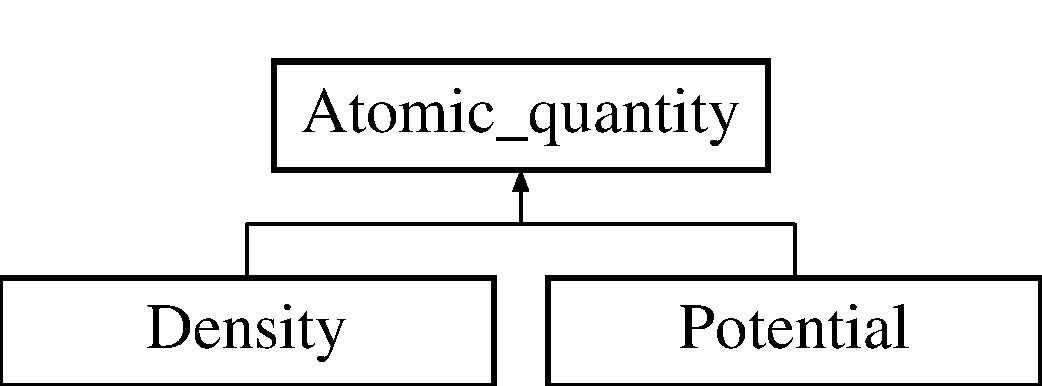
\includegraphics[height=2.000000cm]{classAtomic__quantity}
\end{center}
\end{figure}
\doxysubsection*{Public Member Functions}
\begin{DoxyCompactItemize}
\item 
\mbox{\Hypertarget{classAtomic__quantity_ae304531ff42ea30b543a9fb704e0474b}\label{classAtomic__quantity_ae304531ff42ea30b543a9fb704e0474b}} 
{\bfseries Atomic\+\_\+quantity} (const \mbox{\hyperlink{classCrystal__t}{Crystal\+\_\+t}}$<$ 3, \mbox{\hyperlink{classAtom}{Atom}} $>$ \&cr, const std\+::vector$<$ \mbox{\hyperlink{classLogarithmic__mesh}{Logarithmic\+\_\+mesh}} $>$ \&at\+\_\+meshes)
\item 
\mbox{\Hypertarget{classAtomic__quantity_a5bd9055fdf94e57e54a355d5aa818b6c}\label{classAtomic__quantity_a5bd9055fdf94e57e54a355d5aa818b6c}} 
double {\bfseries operator()} (const G\+S\+L\+::\+Vector \&r)
\item 
\mbox{\Hypertarget{classAtomic__quantity_adfdeab2507a0b975643b53b1df2319b1}\label{classAtomic__quantity_adfdeab2507a0b975643b53b1df2319b1}} 
std\+::vector$<$ double $>$ \& {\bfseries sphere} (const size\+\_\+t i)
\end{DoxyCompactItemize}
\doxysubsection*{Protected Attributes}
\begin{DoxyCompactItemize}
\item 
\mbox{\Hypertarget{classAtomic__quantity_a0fb317241d287bde4bbee6cade84a45f}\label{classAtomic__quantity_a0fb317241d287bde4bbee6cade84a45f}} 
const \mbox{\hyperlink{classCrystal__t}{Crystal\+\_\+t}}$<$ 3, \mbox{\hyperlink{classAtom}{Atom}} $>$ \& {\bfseries cr}
\item 
\mbox{\Hypertarget{classAtomic__quantity_a38619ec6589df0672464f3512243c13f}\label{classAtomic__quantity_a38619ec6589df0672464f3512243c13f}} 
const std\+::vector$<$ \mbox{\hyperlink{classLogarithmic__mesh}{Logarithmic\+\_\+mesh}} $>$ \& {\bfseries at\+\_\+meshes}
\item 
\mbox{\Hypertarget{classAtomic__quantity_a69f4c5e435c8c32883528b7cf2099616}\label{classAtomic__quantity_a69f4c5e435c8c32883528b7cf2099616}} 
std\+::vector$<$ std\+::vector$<$ double $>$ $>$ {\bfseries val}
\end{DoxyCompactItemize}
\doxysubsection*{Friends}
\begin{DoxyCompactItemize}
\item 
\mbox{\Hypertarget{classAtomic__quantity_a678ccaacc1630da5784025bf4ba898bb}\label{classAtomic__quantity_a678ccaacc1630da5784025bf4ba898bb}} 
class {\bfseries Augmented\+\_\+spherical\+\_\+wave}
\end{DoxyCompactItemize}


The documentation for this class was generated from the following file\+:\begin{DoxyCompactItemize}
\item 
atomic\+\_\+quantity.\+h\end{DoxyCompactItemize}

\hypertarget{classAugmented__Bessel}{}\doxysection{Augmented\+\_\+\+Bessel Class Reference}
\label{classAugmented__Bessel}\index{Augmented\_Bessel@{Augmented\_Bessel}}
Inheritance diagram for Augmented\+\_\+\+Bessel\+:\begin{figure}[H]
\begin{center}
\leavevmode
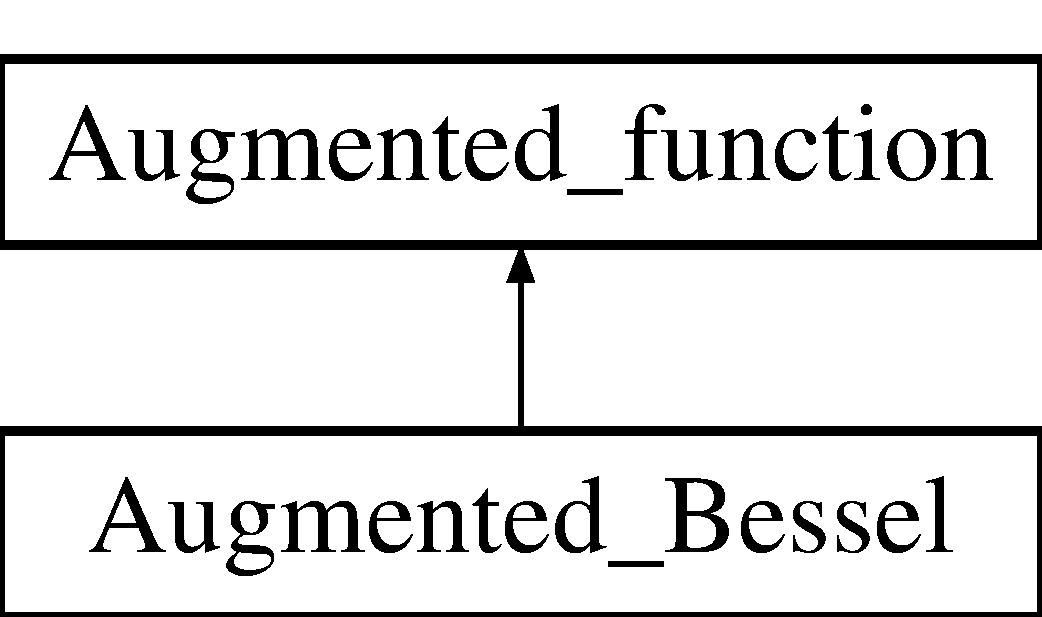
\includegraphics[height=2.000000cm]{classAugmented__Bessel}
\end{center}
\end{figure}
\doxysubsection*{Public Member Functions}
\begin{DoxyCompactItemize}
\item 
\mbox{\Hypertarget{classAugmented__Bessel_a6436bf9381a64f53ce7751e287fdf600}\label{classAugmented__Bessel_a6436bf9381a64f53ce7751e287fdf600}} 
double \& {\bfseries EJ} ()
\item 
\mbox{\Hypertarget{classAugmented__Bessel_afba570534c78adba03db9a98d00aa794}\label{classAugmented__Bessel_afba570534c78adba03db9a98d00aa794}} 
double {\bfseries EJ} () const
\item 
\mbox{\Hypertarget{classAugmented__Bessel_a60211a09e87603960b1f5afa5608192b}\label{classAugmented__Bessel_a60211a09e87603960b1f5afa5608192b}} 
{\bfseries Augmented\+\_\+\+Bessel} (const \mbox{\hyperlink{classAugmented__Bessel}{Augmented\+\_\+\+Bessel}} \&)=default
\item 
\mbox{\Hypertarget{classAugmented__Bessel_a9fb120456c0897692ceb7e74e1846458}\label{classAugmented__Bessel_a9fb120456c0897692ceb7e74e1846458}} 
{\bfseries Augmented\+\_\+\+Bessel} (\mbox{\hyperlink{classAugmented__Bessel}{Augmented\+\_\+\+Bessel}} \&\&)=default
\item 
\mbox{\Hypertarget{classAugmented__Bessel_ac677b36764608a5675856816ab59e95a}\label{classAugmented__Bessel_ac677b36764608a5675856816ab59e95a}} 
{\bfseries Augmented\+\_\+\+Bessel} (const \mbox{\hyperlink{structlm}{lm}} l, const double kappa, const spin s, const \mbox{\hyperlink{classLogarithmic__mesh}{Logarithmic\+\_\+mesh}} \&mesh)
\item 
\mbox{\Hypertarget{classAugmented__Bessel_aa0d2f570116c7ef9a18a1574a36b82ee}\label{classAugmented__Bessel_aa0d2f570116c7ef9a18a1574a36b82ee}} 
\mbox{\hyperlink{classAugmented__Bessel}{Augmented\+\_\+\+Bessel}} \& {\bfseries operator=} (const \mbox{\hyperlink{classAugmented__Bessel}{Augmented\+\_\+\+Bessel}} \&a)=default
\item 
\mbox{\Hypertarget{classAugmented__Bessel_a5692e2965193608da0a90a73a523f766}\label{classAugmented__Bessel_a5692e2965193608da0a90a73a523f766}} 
\mbox{\hyperlink{classAugmented__Bessel}{Augmented\+\_\+\+Bessel}} \& {\bfseries operator=} (\mbox{\hyperlink{classAugmented__Bessel}{Augmented\+\_\+\+Bessel}} \&\&a)=default
\item 
\mbox{\Hypertarget{classAugmented__Bessel_abbf00aa990a7643efcdcb0987217cb96}\label{classAugmented__Bessel_abbf00aa990a7643efcdcb0987217cb96}} 
void {\bfseries update} (std\+::vector$<$ double $>$ \&v, const double en, const bool core) override
\item 
\mbox{\Hypertarget{classAugmented__function_af09e1c0c2c10638bcf058b13e5683daf}\label{classAugmented__function_af09e1c0c2c10638bcf058b13e5683daf}} 
double {\bfseries operator()} (const G\+S\+L\+::\+Vector \&r) const
\item 
\mbox{\Hypertarget{classAugmented__function_a8a340605b6020c71a6fef5a0b8f1251b}\label{classAugmented__function_a8a340605b6020c71a6fef5a0b8f1251b}} 
\mbox{\hyperlink{structlm}{lm}} {\bfseries l} () const
\item 
\mbox{\Hypertarget{classAugmented__function_a5569c661561a7a35bfc59148431726f2}\label{classAugmented__function_a5569c661561a7a35bfc59148431726f2}} 
\mbox{\hyperlink{structlm}{lm}} \& {\bfseries l} ()
\item 
\mbox{\Hypertarget{classAugmented__function_af7f62a70d0293f36ad033b2c3a104a0b}\label{classAugmented__function_af7f62a70d0293f36ad033b2c3a104a0b}} 
double {\bfseries kappa} () const
\item 
\mbox{\Hypertarget{classAugmented__function_a4a3fbc697571fe19a55fb8c8e9409364}\label{classAugmented__function_a4a3fbc697571fe19a55fb8c8e9409364}} 
double \& {\bfseries kappa} ()
\item 
\mbox{\Hypertarget{classAugmented__function_abb7a989dc1a09060bbd9b4bd147df6fe}\label{classAugmented__function_abb7a989dc1a09060bbd9b4bd147df6fe}} 
spin {\bfseries s} () const
\item 
\mbox{\Hypertarget{classAugmented__function_a9fc4ade6a5f4e4a81b8a8577817821f9}\label{classAugmented__function_a9fc4ade6a5f4e4a81b8a8577817821f9}} 
spin \& {\bfseries s} ()
\item 
\mbox{\Hypertarget{classAugmented__function_a52cfb9e9ff3023d4e24a87abfe8433b4}\label{classAugmented__function_a52cfb9e9ff3023d4e24a87abfe8433b4}} 
\mbox{\hyperlink{classLogarithmic__mesh}{Logarithmic\+\_\+mesh}} {\bfseries mesh} () const
\item 
\mbox{\Hypertarget{classAugmented__function_a220205d71230400be2aa804fddb57cfe}\label{classAugmented__function_a220205d71230400be2aa804fddb57cfe}} 
\mbox{\hyperlink{classLogarithmic__mesh}{Logarithmic\+\_\+mesh}} \& {\bfseries mesh} ()
\item 
\mbox{\Hypertarget{classAugmented__function_a27e866d6841096928ea6bba2ebbba613}\label{classAugmented__function_a27e866d6841096928ea6bba2ebbba613}} 
std\+::vector$<$ double $>$ {\bfseries val} () const
\item 
\mbox{\Hypertarget{classAugmented__function_af6b1d2919a83f30567958f99ff528922}\label{classAugmented__function_af6b1d2919a83f30567958f99ff528922}} 
std\+::vector$<$ double $>$ \& {\bfseries val} ()
\item 
\mbox{\Hypertarget{classAugmented__function_a164b2a3ab60e4c89a4ca0b3ac2a011c1}\label{classAugmented__function_a164b2a3ab60e4c89a4ca0b3ac2a011c1}} 
double {\bfseries En} () const
\item 
\mbox{\Hypertarget{classAugmented__function_a655bc4251b7417aa2f82f69b9a839e57}\label{classAugmented__function_a655bc4251b7417aa2f82f69b9a839e57}} 
double \& {\bfseries En} ()
\end{DoxyCompactItemize}
\doxysubsection*{Public Attributes}
\begin{DoxyCompactItemize}
\item 
\mbox{\Hypertarget{classAugmented__function_a68aa65cf592852db5d8aa591faed66a3}\label{classAugmented__function_a68aa65cf592852db5d8aa591faed66a3}} 
\mbox{\hyperlink{structlm}{lm}} {\bfseries l\+\_\+m}
\item 
\mbox{\Hypertarget{classAugmented__function_a084ed4531435bf6c9404f74906bbd675}\label{classAugmented__function_a084ed4531435bf6c9404f74906bbd675}} 
double {\bfseries kappa\+\_\+m}
\item 
\mbox{\Hypertarget{classAugmented__function_ac85d56583de04209d492bb278be988e7}\label{classAugmented__function_ac85d56583de04209d492bb278be988e7}} 
spin {\bfseries s\+\_\+m}
\item 
\mbox{\Hypertarget{classAugmented__function_aa065dcae53178ad8d13373d1a232a3cb}\label{classAugmented__function_aa065dcae53178ad8d13373d1a232a3cb}} 
\mbox{\hyperlink{classLogarithmic__mesh}{Logarithmic\+\_\+mesh}} {\bfseries mesh\+\_\+m}
\item 
\mbox{\Hypertarget{classAugmented__function_a1558390db0687d110c4ef3779dff4a70}\label{classAugmented__function_a1558390db0687d110c4ef3779dff4a70}} 
std\+::vector$<$ double $>$ {\bfseries val\+\_\+m}
\end{DoxyCompactItemize}
\doxysubsection*{Protected Attributes}
\begin{DoxyCompactItemize}
\item 
\mbox{\Hypertarget{classAugmented__function_a87d9bedb5104d916f2d8e4520202ba44}\label{classAugmented__function_a87d9bedb5104d916f2d8e4520202ba44}} 
double {\bfseries En\+\_\+m}
\end{DoxyCompactItemize}


The documentation for this class was generated from the following file\+:\begin{DoxyCompactItemize}
\item 
augmented\+\_\+fun.\+h\end{DoxyCompactItemize}

\hypertarget{classAugmented__function}{}\section{Augmented\+\_\+function Class Reference}
\label{classAugmented__function}\index{Augmented\+\_\+function@{Augmented\+\_\+function}}


{\ttfamily \#include $<$augmented\+\_\+fun.\+h$>$}

Inheritance diagram for Augmented\+\_\+function\+:\begin{figure}[H]
\begin{center}
\leavevmode
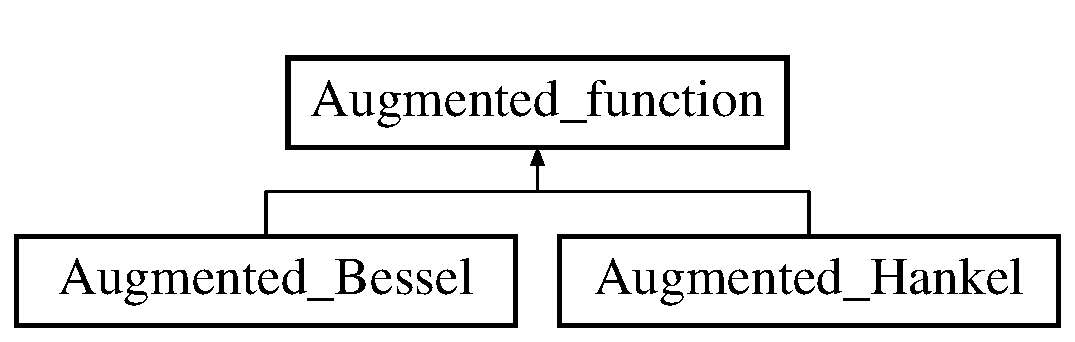
\includegraphics[height=2.000000cm]{classAugmented__function}
\end{center}
\end{figure}
\subsection*{Public Member Functions}
\begin{DoxyCompactItemize}
\item 
\mbox{\Hypertarget{classAugmented__function_ae9be3ac88a8aaffed7deea457a0650f5}\label{classAugmented__function_ae9be3ac88a8aaffed7deea457a0650f5}} 
double \hyperlink{classAugmented__function_ae9be3ac88a8aaffed7deea457a0650f5}{operator()} (const G\+S\+L\+::\+Vector r)
\begin{DoxyCompactList}\small\item\em Obtain value of augmented function at point r. \end{DoxyCompactList}\item 
\mbox{\Hypertarget{classAugmented__function_aaef792b83ff2c7a59cbdbf1b40ff08a7}\label{classAugmented__function_aaef792b83ff2c7a59cbdbf1b40ff08a7}} 
{\bfseries Augmented\+\_\+function} (const \hyperlink{classAugmented__function}{Augmented\+\_\+function} \&)
\item 
\mbox{\Hypertarget{classAugmented__function_a782da1c8f31a70fd897cc8c00bbc0c44}\label{classAugmented__function_a782da1c8f31a70fd897cc8c00bbc0c44}} 
{\bfseries Augmented\+\_\+function} (\hyperlink{classAugmented__function}{Augmented\+\_\+function} \&\&)
\item 
\mbox{\Hypertarget{classAugmented__function_af6f0be4a0f6b78def8f923c8a7daea18}\label{classAugmented__function_af6f0be4a0f6b78def8f923c8a7daea18}} 
{\bfseries Augmented\+\_\+function} (const int n, const \hyperlink{structlm}{lm} l, const double kappa, const G\+S\+L\+::\+Vector center, const \hyperlink{classLogarithmic__mesh}{Logarithmic\+\_\+mesh} mesh)
\item 
\mbox{\Hypertarget{classAugmented__function_aa00aea37783023653cd9880277b51278}\label{classAugmented__function_aa00aea37783023653cd9880277b51278}} 
\hyperlink{classAugmented__function}{Augmented\+\_\+function} \& {\bfseries operator=} (const \hyperlink{classAugmented__function}{Augmented\+\_\+function} \&)
\item 
\mbox{\Hypertarget{classAugmented__function_ad1c67ee06b3e97cb031e69329f94f300}\label{classAugmented__function_ad1c67ee06b3e97cb031e69329f94f300}} 
\hyperlink{classAugmented__function}{Augmented\+\_\+function} \& {\bfseries operator=} (\hyperlink{classAugmented__function}{Augmented\+\_\+function} \&\&)
\item 
\mbox{\Hypertarget{classAugmented__function_a087c956ca3c8cc160ceacaa51e054ee8}\label{classAugmented__function_a087c956ca3c8cc160ceacaa51e054ee8}} 
virtual void {\bfseries update} (std\+::vector$<$ double $>$ v, const double en, const bool core)=0
\end{DoxyCompactItemize}
\subsection*{Public Attributes}
\begin{DoxyCompactItemize}
\item 
\mbox{\Hypertarget{classAugmented__function_a8451882862bc85f60a9160c2bfc5e677}\label{classAugmented__function_a8451882862bc85f60a9160c2bfc5e677}} 
int {\bfseries n}
\item 
\mbox{\Hypertarget{classAugmented__function_a85851e9826059061b94dea2dfeae7b09}\label{classAugmented__function_a85851e9826059061b94dea2dfeae7b09}} 
\hyperlink{structlm}{lm} {\bfseries l}
\item 
\mbox{\Hypertarget{classAugmented__function_acbbd8bf7d17a9557a74f531986f9301b}\label{classAugmented__function_acbbd8bf7d17a9557a74f531986f9301b}} 
double {\bfseries kappa}
\item 
\mbox{\Hypertarget{classAugmented__function_af96cf7923c9d5d656235e3d2c739c99f}\label{classAugmented__function_af96cf7923c9d5d656235e3d2c739c99f}} 
double {\bfseries radius}
\item 
\mbox{\Hypertarget{classAugmented__function_abfe2b7d790f5717ba5f403b6779ff627}\label{classAugmented__function_abfe2b7d790f5717ba5f403b6779ff627}} 
G\+S\+L\+::\+Vector {\bfseries center}
\item 
\mbox{\Hypertarget{classAugmented__function_ad7acfd1cf1c5c5cbca70267348fc10f6}\label{classAugmented__function_ad7acfd1cf1c5c5cbca70267348fc10f6}} 
\hyperlink{classLogarithmic__mesh}{Logarithmic\+\_\+mesh} {\bfseries mesh}
\item 
\mbox{\Hypertarget{classAugmented__function_af11b31e3d3a6e798b6982a135684d4ea}\label{classAugmented__function_af11b31e3d3a6e798b6982a135684d4ea}} 
std\+::vector$<$ double $>$ {\bfseries val}
\end{DoxyCompactItemize}
\subsection*{Friends}
\begin{DoxyCompactItemize}
\item 
\mbox{\Hypertarget{classAugmented__function_a2ce33222aea67403b16a734072c8a1e0}\label{classAugmented__function_a2ce33222aea67403b16a734072c8a1e0}} 
bool {\bfseries operator==} (const \hyperlink{classAugmented__function}{Augmented\+\_\+function} \&a, const \hyperlink{classAugmented__function}{Augmented\+\_\+function} \&b)
\item 
\mbox{\Hypertarget{classAugmented__function_a7e26f4f6e76afdedf16a6b579fb5913e}\label{classAugmented__function_a7e26f4f6e76afdedf16a6b579fb5913e}} 
bool {\bfseries operator!=} (const \hyperlink{classAugmented__function}{Augmented\+\_\+function} \&a, const \hyperlink{classAugmented__function}{Augmented\+\_\+function} \&b)
\end{DoxyCompactItemize}


\subsection{Detailed Description}
Superclass used to describe the general behaviour of an augmented function.~\newline
Contains\+:~\newline
{\bfseries n} -\/ Principal quantum number of the augmented function.~\newline
{\bfseries l} -\/ Combined orbital and angular momentum of the augmented function, l = \{l,m\}.~\newline
{\bfseries kappa} -\/ Energy of waves outside augmentation region, used for matching at sphere boundary.~\newline
{\bfseries radius} -\/ Radius of augmentation sphere.~\newline
{\bfseries center} -\/ Position of the center of the augmentation sphere.~\newline
{\bfseries mesh} -\/ Logarithmic mesh of the augmentation sphere.~\newline
{\bfseries val} -\/ values of the augmented function at the mesh points.~\newline


The documentation for this class was generated from the following files\+:\begin{DoxyCompactItemize}
\item 
augmented\+\_\+fun.\+h\item 
augmented\+\_\+fun.\+cpp\end{DoxyCompactItemize}

\hypertarget{classAugmented__Hankel}{}\section{Augmented\+\_\+\+Hankel Class Reference}
\label{classAugmented__Hankel}\index{Augmented\+\_\+\+Hankel@{Augmented\+\_\+\+Hankel}}


{\ttfamily \#include $<$augmented\+\_\+fun.\+h$>$}

Inheritance diagram for Augmented\+\_\+\+Hankel\+:\begin{figure}[H]
\begin{center}
\leavevmode
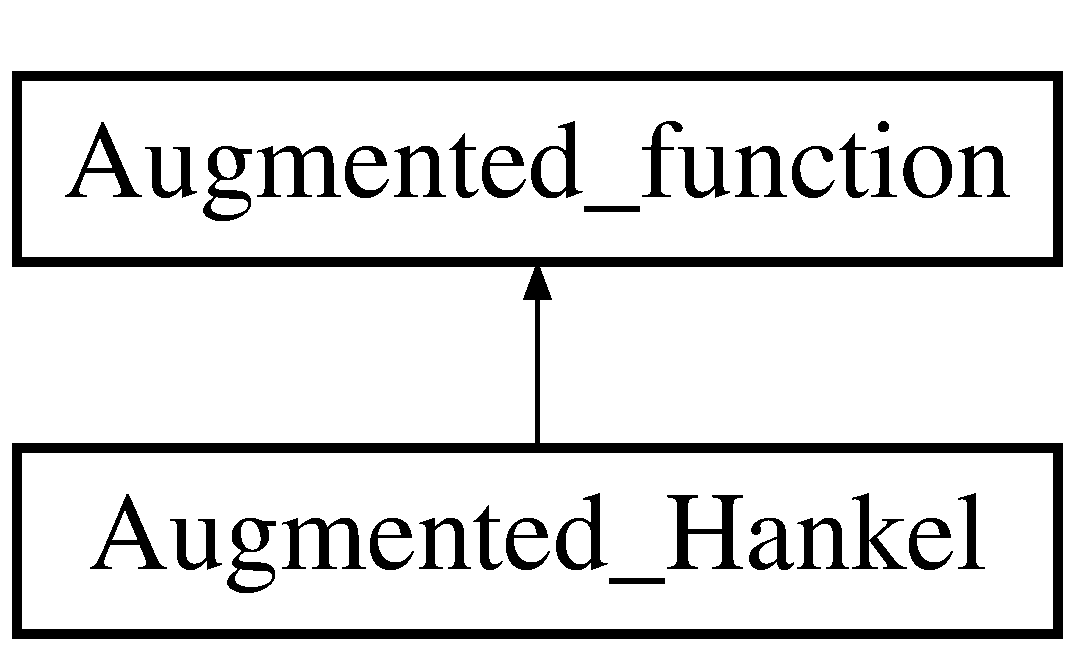
\includegraphics[height=2.000000cm]{classAugmented__Hankel}
\end{center}
\end{figure}
\subsection*{Public Member Functions}
\begin{DoxyCompactItemize}
\item 
\mbox{\Hypertarget{classAugmented__Hankel_ab4abeef208eef604e8f9ec9f962a33c9}\label{classAugmented__Hankel_ab4abeef208eef604e8f9ec9f962a33c9}} 
{\bfseries Augmented\+\_\+\+Hankel} (const \hyperlink{classAugmented__Hankel}{Augmented\+\_\+\+Hankel} \&a)
\item 
\mbox{\Hypertarget{classAugmented__Hankel_a1cd888e6d4bf801283e557c44cbe6e2a}\label{classAugmented__Hankel_a1cd888e6d4bf801283e557c44cbe6e2a}} 
{\bfseries Augmented\+\_\+\+Hankel} (\hyperlink{classAugmented__Hankel}{Augmented\+\_\+\+Hankel} \&\&a)
\item 
\mbox{\Hypertarget{classAugmented__Hankel_af5204b9ee0f1aa65c924f20d671a420c}\label{classAugmented__Hankel_af5204b9ee0f1aa65c924f20d671a420c}} 
{\bfseries Augmented\+\_\+\+Hankel} (const int n, const \hyperlink{structlm}{lm} l, const double kappa, const G\+S\+L\+::\+Vector center, const \hyperlink{classLogarithmic__mesh}{Logarithmic\+\_\+mesh} mesh)
\item 
\mbox{\Hypertarget{classAugmented__Hankel_aeefa7e11896971fb1ea326a4ec5d2d06}\label{classAugmented__Hankel_aeefa7e11896971fb1ea326a4ec5d2d06}} 
\hyperlink{classAugmented__Hankel}{Augmented\+\_\+\+Hankel} \& {\bfseries operator=} (const \hyperlink{classAugmented__Hankel}{Augmented\+\_\+\+Hankel} \&a)
\item 
\mbox{\Hypertarget{classAugmented__Hankel_a9c37b93980c8422d9f15a5d3f8583c5e}\label{classAugmented__Hankel_a9c37b93980c8422d9f15a5d3f8583c5e}} 
\hyperlink{classAugmented__Hankel}{Augmented\+\_\+\+Hankel} \& {\bfseries operator=} (\hyperlink{classAugmented__Hankel}{Augmented\+\_\+\+Hankel} \&\&a)
\item 
\mbox{\Hypertarget{classAugmented__Hankel_ad061623ff90bc66de8c5cf9573f5b72b}\label{classAugmented__Hankel_ad061623ff90bc66de8c5cf9573f5b72b}} 
void {\bfseries update} (std\+::vector$<$ double $>$ v, const double en, const bool core)
\end{DoxyCompactItemize}
\subsection*{Public Attributes}
\begin{DoxyCompactItemize}
\item 
\mbox{\Hypertarget{classAugmented__Hankel_ae2141e9ffe838e2d45fef18514bc3ce6}\label{classAugmented__Hankel_ae2141e9ffe838e2d45fef18514bc3ce6}} 
double {\bfseries EH}
\end{DoxyCompactItemize}


\subsection{Detailed Description}
Class used to represent the augmented Hankel functions.~\newline
Contains\+:~\newline
{\bfseries EH} -\/ Hankel energy, obtained by solving the radial Schrödinger equaiton.~\newline


The documentation for this class was generated from the following files\+:\begin{DoxyCompactItemize}
\item 
augmented\+\_\+fun.\+h\item 
augmented\+\_\+fun.\+cpp\end{DoxyCompactItemize}

\hypertarget{classAugmented__spherical__wave}{}\doxysection{Augmented\+\_\+spherical\+\_\+wave Class Reference}
\label{classAugmented__spherical__wave}\index{Augmented\_spherical\_wave@{Augmented\_spherical\_wave}}
\doxysubsection*{Public Member Functions}
\begin{DoxyCompactItemize}
\item 
\mbox{\Hypertarget{classAugmented__spherical__wave_a3590f819986cb255e98395a65052fac4}\label{classAugmented__spherical__wave_a3590f819986cb255e98395a65052fac4}} 
{\bfseries Augmented\+\_\+spherical\+\_\+wave} (const \mbox{\hyperlink{classAugmented__spherical__wave}{Augmented\+\_\+spherical\+\_\+wave}} \&)=default
\item 
\mbox{\Hypertarget{classAugmented__spherical__wave_a90288e34627a1072c8581753af7e15a9}\label{classAugmented__spherical__wave_a90288e34627a1072c8581753af7e15a9}} 
{\bfseries Augmented\+\_\+spherical\+\_\+wave} (\mbox{\hyperlink{classAugmented__spherical__wave}{Augmented\+\_\+spherical\+\_\+wave}} \&\&)=default
\item 
\mbox{\Hypertarget{classAugmented__spherical__wave_a27480f16a5d4d0a5341d97736bc1c8cf}\label{classAugmented__spherical__wave_a27480f16a5d4d0a5341d97736bc1c8cf}} 
{\bfseries Augmented\+\_\+spherical\+\_\+wave} (\mbox{\hyperlink{classSite__t}{Site\+\_\+t}}$<$ 3 $>$ center, double kappa, \mbox{\hyperlink{structlm}{lm}} l, spin s, bool core\+\_\+state=false)
\item 
\mbox{\Hypertarget{classAugmented__spherical__wave_a25f4adef095771878038446faabad089}\label{classAugmented__spherical__wave_a25f4adef095771878038446faabad089}} 
\mbox{\hyperlink{classAugmented__spherical__wave}{Augmented\+\_\+spherical\+\_\+wave}} \& {\bfseries operator=} (const \mbox{\hyperlink{classAugmented__spherical__wave}{Augmented\+\_\+spherical\+\_\+wave}} \&)=default
\item 
\mbox{\Hypertarget{classAugmented__spherical__wave_ab1125d706552f1cfce1897a484aaa9b3}\label{classAugmented__spherical__wave_ab1125d706552f1cfce1897a484aaa9b3}} 
\mbox{\hyperlink{classAugmented__spherical__wave}{Augmented\+\_\+spherical\+\_\+wave}} \& {\bfseries operator=} (\mbox{\hyperlink{classAugmented__spherical__wave}{Augmented\+\_\+spherical\+\_\+wave}} \&\&)=default
\item 
\mbox{\Hypertarget{classAugmented__spherical__wave_a39c7fe6a3f7a752adb6fd581b94ef533}\label{classAugmented__spherical__wave_a39c7fe6a3f7a752adb6fd581b94ef533}} 
\mbox{\hyperlink{classSite__t}{Site\+\_\+t}}$<$ 3 $>$ \& {\bfseries center} ()
\item 
\mbox{\Hypertarget{classAugmented__spherical__wave_a6c52889c8c1397bdcf8e0f2b74830eb1}\label{classAugmented__spherical__wave_a6c52889c8c1397bdcf8e0f2b74830eb1}} 
\mbox{\hyperlink{classSite__t}{Site\+\_\+t}}$<$ 3 $>$ {\bfseries center} () const
\item 
\mbox{\Hypertarget{classAugmented__spherical__wave_a1a5d94905faa383336a1b1fb45e71682}\label{classAugmented__spherical__wave_a1a5d94905faa383336a1b1fb45e71682}} 
double {\bfseries kappa} () const
\item 
\mbox{\Hypertarget{classAugmented__spherical__wave_a805aadb619c60113ef9715dd65094ecc}\label{classAugmented__spherical__wave_a805aadb619c60113ef9715dd65094ecc}} 
\mbox{\hyperlink{structlm}{lm}} {\bfseries l} () const
\item 
\mbox{\Hypertarget{classAugmented__spherical__wave_ac540c393892f68a4abde993cbac880ac}\label{classAugmented__spherical__wave_ac540c393892f68a4abde993cbac880ac}} 
spin {\bfseries s} () const
\item 
\mbox{\Hypertarget{classAugmented__spherical__wave_a8bb547e42384ec44caac77ec584f0cfb}\label{classAugmented__spherical__wave_a8bb547e42384ec44caac77ec584f0cfb}} 
bool {\bfseries core\+\_\+state} () const
\end{DoxyCompactItemize}


The documentation for this class was generated from the following file\+:\begin{DoxyCompactItemize}
\item 
augmented\+\_\+spherical\+\_\+wave.\+h\end{DoxyCompactItemize}

\hypertarget{classBessel__function}{}\section{Bessel\+\_\+function Class Reference}
\label{classBessel__function}\index{Bessel\+\_\+function@{Bessel\+\_\+function}}
Inheritance diagram for Bessel\+\_\+function\+:\begin{figure}[H]
\begin{center}
\leavevmode
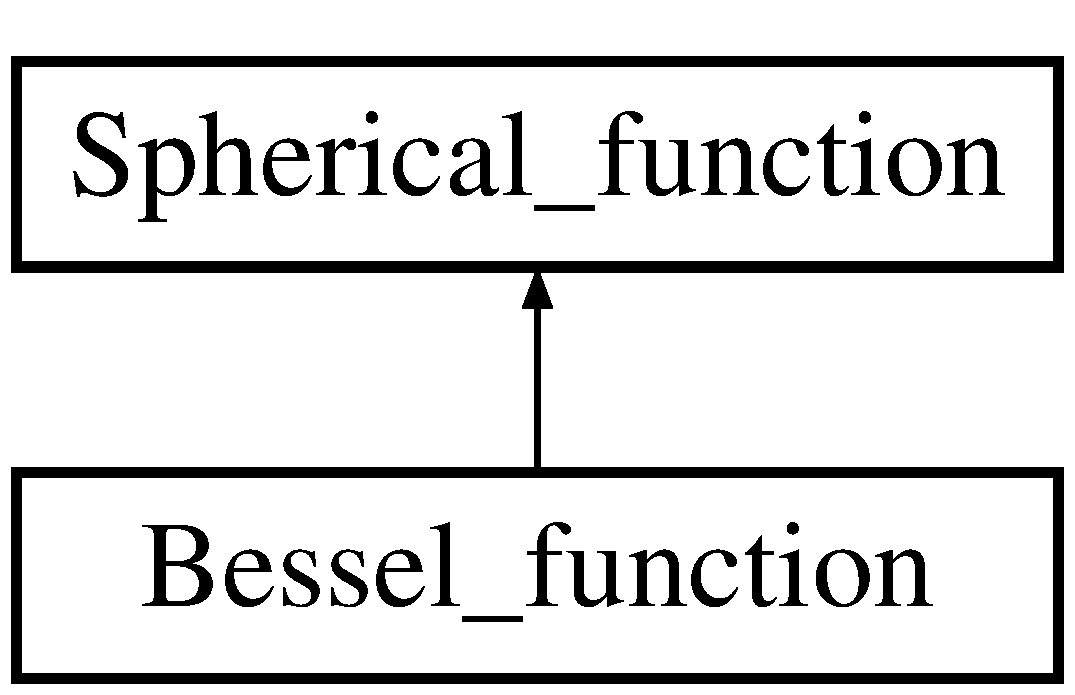
\includegraphics[height=2.000000cm]{classBessel__function}
\end{center}
\end{figure}
\subsection*{Public Member Functions}
\begin{DoxyCompactItemize}
\item 
\mbox{\Hypertarget{classBessel__function_acd510b87d95ff582c967e1dbaf49a4b3}\label{classBessel__function_acd510b87d95ff582c967e1dbaf49a4b3}} 
{\bfseries Bessel\+\_\+function} (const \hyperlink{structlm}{lm} l)
\item 
\mbox{\Hypertarget{classBessel__function_a7af0b3054971c3c7027e2076da112c2c}\label{classBessel__function_a7af0b3054971c3c7027e2076da112c2c}} 
double {\bfseries operator()} (const double x)
\end{DoxyCompactItemize}
\subsection*{Additional Inherited Members}


The documentation for this class was generated from the following files\+:\begin{DoxyCompactItemize}
\item 
spherical\+\_\+fun.\+h\item 
spherical\+\_\+fun.\+cpp\end{DoxyCompactItemize}

\hypertarget{classBloch__sum}{}\section{Bloch\+\_\+sum Class Reference}
\label{classBloch__sum}\index{Bloch\+\_\+sum@{Bloch\+\_\+sum}}
\subsection*{Public Member Functions}
\begin{DoxyCompactItemize}
\item 
\mbox{\Hypertarget{classBloch__sum_ad0b17c6c7ab656afa9ad65083ef479d1}\label{classBloch__sum_ad0b17c6c7ab656afa9ad65083ef479d1}} 
{\bfseries Bloch\+\_\+sum} (const \hyperlink{structlm}{lm} l, const double kappa, const \hyperlink{classCrystal}{Crystal} c)
\item 
\mbox{\Hypertarget{classBloch__sum_aed260ebecdae29d493ed57cb387a3cdf}\label{classBloch__sum_aed260ebecdae29d493ed57cb387a3cdf}} 
G\+S\+L\+::\+Complex {\bfseries hankel\+\_\+envelope} (const G\+S\+L\+::\+Vector \&tau, const G\+S\+L\+::\+Vector \&kp)
\item 
\mbox{\Hypertarget{classBloch__sum_a5a1979ae3a3adefe783068b965f45774}\label{classBloch__sum_a5a1979ae3a3adefe783068b965f45774}} 
G\+S\+L\+::\+Complex {\bfseries hankel\+\_\+envelope\+\_\+dot} (const G\+S\+L\+::\+Vector \&tau, const G\+S\+L\+::\+Vector \&kp)
\end{DoxyCompactItemize}


The documentation for this class was generated from the following files\+:\begin{DoxyCompactItemize}
\item 
bloch\+\_\+sum.\+h\item 
bloch\+\_\+sum.\+cpp\end{DoxyCompactItemize}

\hypertarget{classBloch__summed__structure__constant}{}\section{Bloch\+\_\+summed\+\_\+structure\+\_\+constant Class Reference}
\label{classBloch__summed__structure__constant}\index{Bloch\+\_\+summed\+\_\+structure\+\_\+constant@{Bloch\+\_\+summed\+\_\+structure\+\_\+constant}}


{\ttfamily \#include $<$structure\+\_\+const.\+h$>$}

\subsection*{Public Member Functions}
\begin{DoxyCompactItemize}
\item 
\mbox{\Hypertarget{classBloch__summed__structure__constant_a76a707b0527f92350141011264fa1f29}\label{classBloch__summed__structure__constant_a76a707b0527f92350141011264fa1f29}} 
{\bfseries Bloch\+\_\+summed\+\_\+structure\+\_\+constant} (int l\+\_\+low, int l\+\_\+int, double kappa, \hyperlink{classCrystal}{Crystal} \&c, \hyperlink{structlm}{lm} l1, \hyperlink{structlm}{lm} l2)
\item 
\mbox{\Hypertarget{classBloch__summed__structure__constant_a6a12a7cf46a1a9b52ac6852df7a87c91}\label{classBloch__summed__structure__constant_a6a12a7cf46a1a9b52ac6852df7a87c91}} 
{\bfseries Bloch\+\_\+summed\+\_\+structure\+\_\+constant} (int l\+\_\+low, int l\+\_\+int, \hyperlink{classCrystal}{Crystal} \&c, \hyperlink{structlm}{lm} l1, \hyperlink{structlm}{lm} l2)
\item 
\mbox{\Hypertarget{classBloch__summed__structure__constant_a9ec01b0c1f625a2beec618d6da838b48}\label{classBloch__summed__structure__constant_a9ec01b0c1f625a2beec618d6da838b48}} 
{\bfseries Bloch\+\_\+summed\+\_\+structure\+\_\+constant} (int l\+\_\+low, \hyperlink{classCrystal}{Crystal} \&c, \hyperlink{structlm}{lm} l1, \hyperlink{structlm}{lm} l2)
\item 
\mbox{\Hypertarget{classBloch__summed__structure__constant_a5a0864288d912b93ac8cdb10f55f338d}\label{classBloch__summed__structure__constant_a5a0864288d912b93ac8cdb10f55f338d}} 
{\bfseries Bloch\+\_\+summed\+\_\+structure\+\_\+constant} (\hyperlink{classCrystal}{Crystal} \&c, \hyperlink{structlm}{lm} l1, \hyperlink{structlm}{lm} l2)
\item 
\mbox{\Hypertarget{classBloch__summed__structure__constant_a43503e7c75fb86c7646ec9373c7bd5fc}\label{classBloch__summed__structure__constant_a43503e7c75fb86c7646ec9373c7bd5fc}} 
G\+S\+L\+::\+Complex \hyperlink{classBloch__summed__structure__constant_a43503e7c75fb86c7646ec9373c7bd5fc}{evaluate} (const G\+S\+L\+::\+Vector \&tau, const G\+S\+L\+::\+Vector \&kp)
\begin{DoxyCompactList}\small\item\em Evaluate the Bloch summed structure constant at point tau for k-\/point kp. \end{DoxyCompactList}\item 
\mbox{\Hypertarget{classBloch__summed__structure__constant_abc1d8c593a9f4e6dca95f969847dfe67}\label{classBloch__summed__structure__constant_abc1d8c593a9f4e6dca95f969847dfe67}} 
G\+S\+L\+::\+Complex \hyperlink{classBloch__summed__structure__constant_abc1d8c593a9f4e6dca95f969847dfe67}{dot\+\_\+evaluate} (const G\+S\+L\+::\+Vector \&tau, const G\+S\+L\+::\+Vector \&kp)
\begin{DoxyCompactList}\small\item\em Evaluate the energy derivative of the Bloch summed structure constant at point tau for k-\/point kp. \end{DoxyCompactList}\end{DoxyCompactItemize}
\subsection*{Friends}
\begin{DoxyCompactItemize}
\item 
\mbox{\Hypertarget{classBloch__summed__structure__constant_a842c35198ecf8ef46be7efe1471b4809}\label{classBloch__summed__structure__constant_a842c35198ecf8ef46be7efe1471b4809}} 
std\+::ostream \& {\bfseries operator$<$$<$} (std\+::ostream \&, const \hyperlink{classBloch__summed__structure__constant}{Bloch\+\_\+summed\+\_\+structure\+\_\+constant} \&)
\end{DoxyCompactItemize}


\subsection{Detailed Description}
A class for representing Bloch summed structure constants~\newline
Contains\+:~\newline
{\bfseries l\+\_\+int} -\/ Maximum orbital angular momentum to be included for Bessel expansions~\newline
 {\bfseries l\+\_\+low} -\/ Maximumm orbital angular momentum to be included for Hankel expansions~\newline
 {\bfseries l1}, {\bfseries l2} -\/ Orbital angular momenta to couple via the structure constant~\newline
{\bfseries kappa} -\/ Energy parameter used (usually kappa$^\wedge$2 = -\/0.\+015)~\newline
{\bfseries c} -\/ Unit cell of the crystal.~\newline


The documentation for this class was generated from the following files\+:\begin{DoxyCompactItemize}
\item 
structure\+\_\+const.\+h\item 
structure\+\_\+const.\+cpp\end{DoxyCompactItemize}

\hypertarget{classCrystal}{}\section{Crystal Class Reference}
\label{classCrystal}\index{Crystal@{Crystal}}


{\ttfamily \#include $<$crystal.\+h$>$}

\subsection*{Public Member Functions}
\begin{DoxyCompactItemize}
\item 
\mbox{\Hypertarget{classCrystal_af60ff2a10146e75a52e6df02c54f35d9}\label{classCrystal_af60ff2a10146e75a52e6df02c54f35d9}} 
size\+\_\+t {\bfseries calc\+\_\+nk} (double tol, double kappa, \hyperlink{structlm}{lm} l)
\item 
\mbox{\Hypertarget{classCrystal_af1c7ecea434e2fd23179c31f4dc293ab}\label{classCrystal_af1c7ecea434e2fd23179c31f4dc293ab}} 
size\+\_\+t {\bfseries calc\+\_\+nr} (double tol, double kappa, \hyperlink{structlm}{lm} l)
\item 
\mbox{\Hypertarget{classCrystal_a7d5661dea0deafd0ec6c9e473fc64903}\label{classCrystal_a7d5661dea0deafd0ec6c9e473fc64903}} 
void {\bfseries calc\+\_\+\+Kn} (size\+\_\+t num)
\item 
\mbox{\Hypertarget{classCrystal_a49ec1aa8a9072ed17bd2fe72fa1a17f5}\label{classCrystal_a49ec1aa8a9072ed17bd2fe72fa1a17f5}} 
void {\bfseries calc\+\_\+\+Rn} (size\+\_\+t num)
\item 
\mbox{\Hypertarget{classCrystal_a48b64a146c0a7d5c535d9810f9a4db0f}\label{classCrystal_a48b64a146c0a7d5c535d9810f9a4db0f}} 
{\bfseries Crystal} (double \&a)
\item 
\mbox{\Hypertarget{classCrystal_a833d7b176886858f4c60783e8a206fca}\label{classCrystal_a833d7b176886858f4c60783e8a206fca}} 
{\bfseries Crystal} (const double \&a)
\item 
\mbox{\Hypertarget{classCrystal_ad3d2d5e6685320d29315645218d9ef3e}\label{classCrystal_ad3d2d5e6685320d29315645218d9ef3e}} 
{\bfseries Crystal} (double \&a, double \&b, double \&c)
\item 
\mbox{\Hypertarget{classCrystal_a7fbd1876776468459c219f3f2682151a}\label{classCrystal_a7fbd1876776468459c219f3f2682151a}} 
{\bfseries Crystal} (const double \&a, const double \&b, const double \&c)
\item 
\mbox{\Hypertarget{classCrystal_a8ce1dcbea5d7044e7c76036539e457ef}\label{classCrystal_a8ce1dcbea5d7044e7c76036539e457ef}} 
{\bfseries Crystal} (G\+S\+L\+::\+Vector \&a, G\+S\+L\+::\+Vector \&b, G\+S\+L\+::\+Vector \&c)
\item 
\mbox{\Hypertarget{classCrystal_a731c41bd979ebae689c9c37546ebcb94}\label{classCrystal_a731c41bd979ebae689c9c37546ebcb94}} 
{\bfseries Crystal} (const G\+S\+L\+::\+Vector \&a, const G\+S\+L\+::\+Vector \&b, const G\+S\+L\+::\+Vector \&c)
\item 
\mbox{\Hypertarget{classCrystal_a5b6c668fc1d66d1069ed4f24348317a9}\label{classCrystal_a5b6c668fc1d66d1069ed4f24348317a9}} 
void {\bfseries add\+\_\+atoms} (const std\+::vector$<$ \hyperlink{classAtom}{Atom} $>$ \&v)
\item 
\mbox{\Hypertarget{classCrystal_ad3d68928046871d142b88bdc98219ff2}\label{classCrystal_ad3d68928046871d142b88bdc98219ff2}} 
G\+S\+L\+::\+Vector \& {\bfseries get\+\_\+\+Rn} (const size\+\_\+t \&i)
\item 
\mbox{\Hypertarget{classCrystal_a87bfc2e2f34dd9c1344ed1aeb4f56d8c}\label{classCrystal_a87bfc2e2f34dd9c1344ed1aeb4f56d8c}} 
std\+::vector$<$ std\+::vector$<$ \hyperlink{classAtom}{Atom} $>$ $>$ {\bfseries calc\+\_\+nearest\+\_\+neighbours} ()
\end{DoxyCompactItemize}
\subsection*{Public Attributes}
\begin{DoxyCompactItemize}
\item 
\mbox{\Hypertarget{classCrystal_ad8a47a7a1bff618d0f8086b0f6dc8923}\label{classCrystal_ad8a47a7a1bff618d0f8086b0f6dc8923}} 
std\+::vector$<$ G\+S\+L\+::\+Vector $>$ {\bfseries Rn\+\_\+vecs}
\item 
\mbox{\Hypertarget{classCrystal_abe2274d5f8cb3f04b86b2f12a41be29e}\label{classCrystal_abe2274d5f8cb3f04b86b2f12a41be29e}} 
std\+::vector$<$ G\+S\+L\+::\+Vector $>$ {\bfseries Kn\+\_\+vecs}
\item 
\mbox{\Hypertarget{classCrystal_a40f8e54181ebde8cbfd5cdfca4c566a0}\label{classCrystal_a40f8e54181ebde8cbfd5cdfca4c566a0}} 
\hyperlink{classLattice}{Lattice} {\bfseries lat}
\item 
\mbox{\Hypertarget{classCrystal_a3bf1b97769d7ebb26f5b0947887c0b3f}\label{classCrystal_a3bf1b97769d7ebb26f5b0947887c0b3f}} 
std\+::vector$<$ \hyperlink{classAtom}{Atom} $>$ {\bfseries atoms}
\item 
\mbox{\Hypertarget{classCrystal_a0a6ca7dd06a76590ce88bfd9140f9441}\label{classCrystal_a0a6ca7dd06a76590ce88bfd9140f9441}} 
double {\bfseries volume}
\item 
\mbox{\Hypertarget{classCrystal_a34c90595f775055b60f929831550d91b}\label{classCrystal_a34c90595f775055b60f929831550d91b}} 
double {\bfseries bz\+\_\+volume}
\end{DoxyCompactItemize}


\subsection{Detailed Description}
Class used to describe the structure of a crystal.~\newline
Contains\+:~\newline
{\bfseries Rn\+\_\+vecs} -\/ \hyperlink{classLattice}{Lattice} vectors of the crystal (up to a maximum lentgh).~\newline
{\bfseries Kn\+\_\+vecs} -\/ Reciprocal lattice vectors of the crystal (up to a maximum length).~\newline
{\bfseries lat} -\/ The lattice of the crystal.~\newline
{\bfseries atoms} -\/ The atoms in the unit cell of the crystal (the base of the crystal).~\newline


The documentation for this class was generated from the following files\+:\begin{DoxyCompactItemize}
\item 
crystal.\+h\item 
crystal.\+cpp\end{DoxyCompactItemize}

\hypertarget{classDensity}{}\section{Density Class Reference}
\label{classDensity}\index{Density@{Density}}


{\ttfamily \#include $<$atomic\+\_\+quantity.\+h$>$}

Inheritance diagram for Density\+:\begin{figure}[H]
\begin{center}
\leavevmode
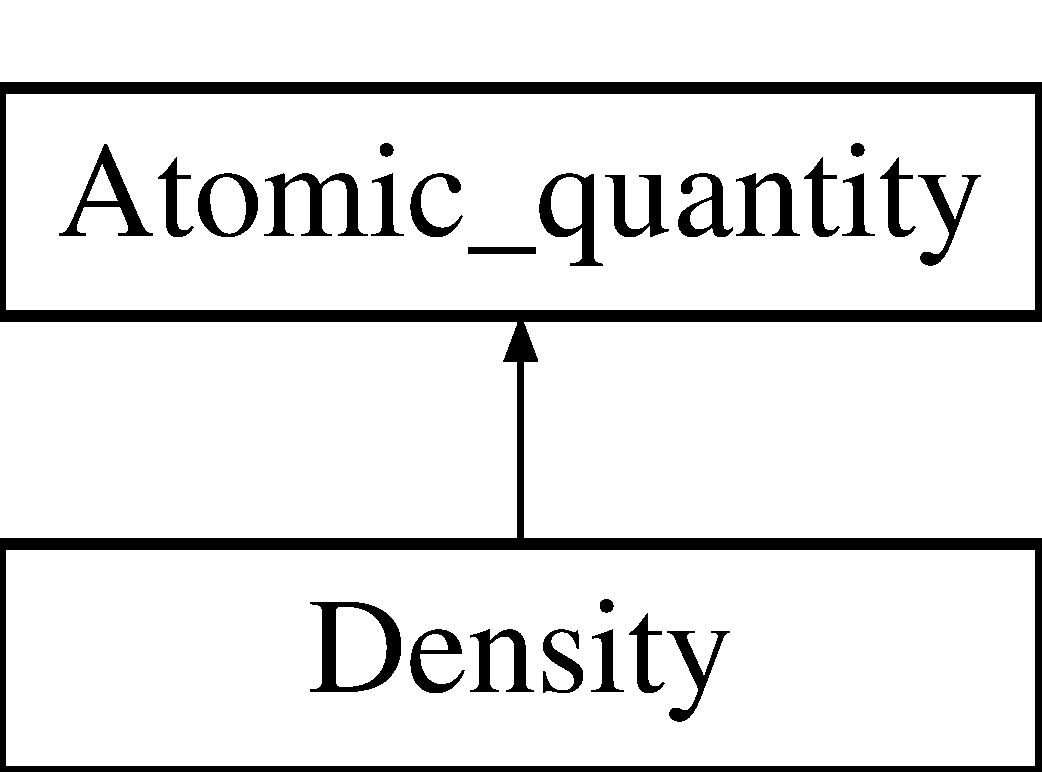
\includegraphics[height=2.000000cm]{classDensity}
\end{center}
\end{figure}
\subsection*{Public Member Functions}
\begin{DoxyCompactItemize}
\item 
\mbox{\Hypertarget{classDensity_aa6d4e3c21169b9e4621ce23e7691068f}\label{classDensity_aa6d4e3c21169b9e4621ce23e7691068f}} 
{\bfseries Density} (\hyperlink{classDensity}{Density} \&)=default
\item 
\mbox{\Hypertarget{classDensity_aba98ae4c1dc9fbbb40754ccd09cb4f3e}\label{classDensity_aba98ae4c1dc9fbbb40754ccd09cb4f3e}} 
{\bfseries Density} (\hyperlink{classDensity}{Density} \&\&)=default
\item 
\mbox{\Hypertarget{classDensity_a86dfd88c2a8c52f356ac743e44b0cca9}\label{classDensity_a86dfd88c2a8c52f356ac743e44b0cca9}} 
\hyperlink{classDensity}{Density} \& {\bfseries operator=} (const \hyperlink{classDensity}{Density} \&)=default
\item 
\mbox{\Hypertarget{classDensity_a6128faad5c75a914d40222844b324a1e}\label{classDensity_a6128faad5c75a914d40222844b324a1e}} 
\hyperlink{classDensity}{Density} \& {\bfseries operator=} (\hyperlink{classDensity}{Density} \&\&)=default
\item 
\mbox{\Hypertarget{classDensity_ae48ea1fc60168a20bc97f20eaef329bb}\label{classDensity_ae48ea1fc60168a20bc97f20eaef329bb}} 
{\bfseries Density} (std\+::vector$<$ \hyperlink{classAtom}{Atom} $>$ \&atoms)
\end{DoxyCompactItemize}
\subsection*{Additional Inherited Members}


\subsection{Detailed Description}
Class used for representing the electronic charge density.~\newline
Contains\+:~\newline
{\bfseries valence} -\/ \hyperlink{classDensity}{Density} gengerated by valence electrons.~\newline
{\bfseries core} -\/ \hyperlink{classDensity}{Density} generated by core electrons.~\newline


The documentation for this class was generated from the following files\+:\begin{DoxyCompactItemize}
\item 
atomic\+\_\+quantity.\+h\item 
atomic\+\_\+quantity.\+cpp\end{DoxyCompactItemize}

\hypertarget{classEffective__potential}{}\doxysection{Effective\+\_\+potential Class Reference}
\label{classEffective__potential}\index{Effective\_potential@{Effective\_potential}}


The documentation for this class was generated from the following file\+:\begin{DoxyCompactItemize}
\item 
eff\+\_\+pot.\+h\end{DoxyCompactItemize}

\hypertarget{classEnvelope__Bessel}{}\doxysection{Envelope\+\_\+\+Bessel Class Reference}
\label{classEnvelope__Bessel}\index{Envelope\_Bessel@{Envelope\_Bessel}}
Inheritance diagram for Envelope\+\_\+\+Bessel\+:\begin{figure}[H]
\begin{center}
\leavevmode
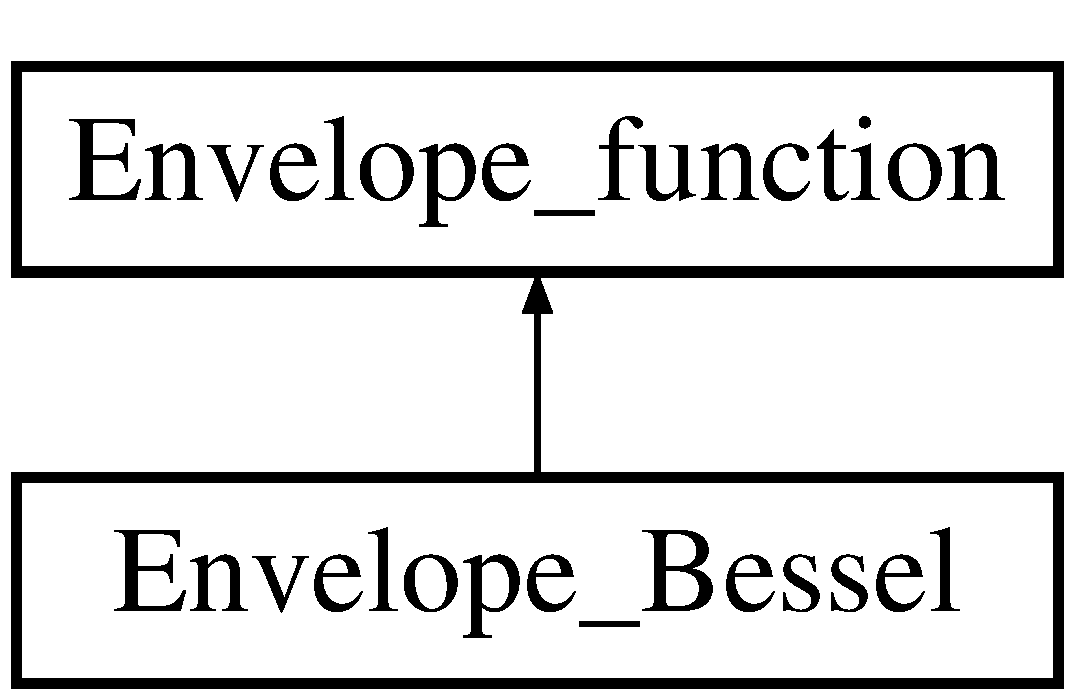
\includegraphics[height=2.000000cm]{classEnvelope__Bessel}
\end{center}
\end{figure}
\doxysubsection*{Public Member Functions}
\begin{DoxyCompactItemize}
\item 
\mbox{\Hypertarget{classEnvelope__Bessel_ab0423f7c349d4e51186553a6c6a527fa}\label{classEnvelope__Bessel_ab0423f7c349d4e51186553a6c6a527fa}} 
{\bfseries Envelope\+\_\+\+Bessel} (\mbox{\hyperlink{structlm}{lm}} l\+\_\+n, double kappa\+\_\+n)
\item 
\mbox{\Hypertarget{classEnvelope__Bessel_a8e2399261bcbbfddb84a7f9ea6c7aa32}\label{classEnvelope__Bessel_a8e2399261bcbbfddb84a7f9ea6c7aa32}} 
double {\bfseries barred\+\_\+fun} (const double x) const override
\item 
\mbox{\Hypertarget{classEnvelope__function_a21a876fdc33d23725bdb25990d3f6e6a}\label{classEnvelope__function_a21a876fdc33d23725bdb25990d3f6e6a}} 
double {\bfseries operator()} (const G\+S\+L\+::\+Vector r)
\item 
\mbox{\Hypertarget{classEnvelope__function_a85cd53700d4090e4c0f6dc2e67d7bb42}\label{classEnvelope__function_a85cd53700d4090e4c0f6dc2e67d7bb42}} 
double {\bfseries kappa} () const
\item 
\mbox{\Hypertarget{classEnvelope__function_a94d64257a361bdbf28e2dd525346ceb7}\label{classEnvelope__function_a94d64257a361bdbf28e2dd525346ceb7}} 
double \& {\bfseries kappa} ()
\item 
\mbox{\Hypertarget{classEnvelope__function_a44ac505a0bc963b230a94c0b25d1a61f}\label{classEnvelope__function_a44ac505a0bc963b230a94c0b25d1a61f}} 
\mbox{\hyperlink{structlm}{lm}} {\bfseries l} () const
\item 
\mbox{\Hypertarget{classEnvelope__function_a5caa2943467fe3e75bf8047ef062f196}\label{classEnvelope__function_a5caa2943467fe3e75bf8047ef062f196}} 
\mbox{\hyperlink{structlm}{lm}} \& {\bfseries l} ()
\end{DoxyCompactItemize}
\doxysubsection*{Protected Attributes}
\begin{DoxyCompactItemize}
\item 
\mbox{\Hypertarget{classEnvelope__function_a41518f3ca4477df62028318dd6c88f86}\label{classEnvelope__function_a41518f3ca4477df62028318dd6c88f86}} 
\mbox{\hyperlink{structlm}{lm}} {\bfseries l\+\_\+m}
\item 
\mbox{\Hypertarget{classEnvelope__function_a14925f5c7ac21806a89fd2b7049d47ed}\label{classEnvelope__function_a14925f5c7ac21806a89fd2b7049d47ed}} 
double {\bfseries kappa\+\_\+m}
\end{DoxyCompactItemize}
\doxysubsection*{Friends}
\begin{DoxyCompactItemize}
\item 
\mbox{\Hypertarget{classEnvelope__Bessel_ae3e190b6f367e1f0fd40f9b4318f422e}\label{classEnvelope__Bessel_ae3e190b6f367e1f0fd40f9b4318f422e}} 
double {\bfseries atomic\+\_\+integral} (const \mbox{\hyperlink{classEnvelope__Hankel}{Envelope\+\_\+\+Hankel}} \&H1, const \mbox{\hyperlink{classEnvelope__Bessel}{Envelope\+\_\+\+Bessel}} \&J2, const double rs)
\item 
\mbox{\Hypertarget{classEnvelope__Bessel_a7edfba8f6f921b0b9523e7aaed9ee6ea}\label{classEnvelope__Bessel_a7edfba8f6f921b0b9523e7aaed9ee6ea}} 
double {\bfseries atomic\+\_\+integral} (const \mbox{\hyperlink{classEnvelope__Bessel}{Envelope\+\_\+\+Bessel}} \&J1, const \mbox{\hyperlink{classEnvelope__Bessel}{Envelope\+\_\+\+Bessel}} \&J2, const double rs)
\item 
\mbox{\Hypertarget{classEnvelope__Bessel_a60510a52b89da071bda3a777586b0a41}\label{classEnvelope__Bessel_a60510a52b89da071bda3a777586b0a41}} 
double {\bfseries off\+\_\+atomic\+\_\+integral} (const \mbox{\hyperlink{classEnvelope__Hankel}{Envelope\+\_\+\+Hankel}} \&H1, const \mbox{\hyperlink{classEnvelope__Bessel}{Envelope\+\_\+\+Bessel}} \&J2, const double rs)
\end{DoxyCompactItemize}


The documentation for this class was generated from the following file\+:\begin{DoxyCompactItemize}
\item 
envelope\+\_\+fun.\+h\end{DoxyCompactItemize}

\hypertarget{classEnvelope__function}{}\doxysection{Envelope\+\_\+function Class Reference}
\label{classEnvelope__function}\index{Envelope\_function@{Envelope\_function}}
Inheritance diagram for Envelope\+\_\+function\+:\begin{figure}[H]
\begin{center}
\leavevmode
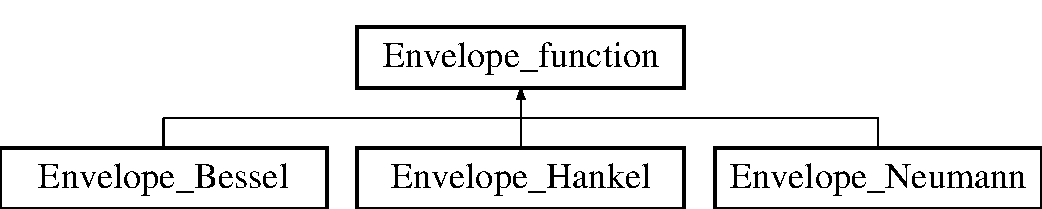
\includegraphics[height=2.000000cm]{classEnvelope__function}
\end{center}
\end{figure}
\doxysubsection*{Public Member Functions}
\begin{DoxyCompactItemize}
\item 
\mbox{\Hypertarget{classEnvelope__function_a4075694daf40dec43b18a7cce9551cfc}\label{classEnvelope__function_a4075694daf40dec43b18a7cce9551cfc}} 
{\bfseries Envelope\+\_\+function} (\mbox{\hyperlink{structlm}{lm}} l\+\_\+n, double kappa\+\_\+n)
\item 
\mbox{\Hypertarget{classEnvelope__function_a2870da644b995b082437c1774f079774}\label{classEnvelope__function_a2870da644b995b082437c1774f079774}} 
{\bfseries Envelope\+\_\+function} (const \mbox{\hyperlink{classEnvelope__function}{Envelope\+\_\+function}} \&)=default
\item 
\mbox{\Hypertarget{classEnvelope__function_a2b4980b7e5866a851316ce87c0edeb75}\label{classEnvelope__function_a2b4980b7e5866a851316ce87c0edeb75}} 
{\bfseries Envelope\+\_\+function} (\mbox{\hyperlink{classEnvelope__function}{Envelope\+\_\+function}} \&\&)=default
\item 
\mbox{\Hypertarget{classEnvelope__function_a5e7ade4f940bd982224c15305b785b80}\label{classEnvelope__function_a5e7ade4f940bd982224c15305b785b80}} 
\mbox{\hyperlink{classEnvelope__function}{Envelope\+\_\+function}} \& {\bfseries operator=} (const \mbox{\hyperlink{classEnvelope__function}{Envelope\+\_\+function}} \&)=default
\item 
\mbox{\Hypertarget{classEnvelope__function_a0e8804f8b1405973c45f991f88ce4cb8}\label{classEnvelope__function_a0e8804f8b1405973c45f991f88ce4cb8}} 
\mbox{\hyperlink{classEnvelope__function}{Envelope\+\_\+function}} \& {\bfseries operator=} (\mbox{\hyperlink{classEnvelope__function}{Envelope\+\_\+function}} \&\&)=default
\item 
\mbox{\Hypertarget{classEnvelope__function_a21a876fdc33d23725bdb25990d3f6e6a}\label{classEnvelope__function_a21a876fdc33d23725bdb25990d3f6e6a}} 
double {\bfseries operator()} (const G\+S\+L\+::\+Vector r)
\item 
\mbox{\Hypertarget{classEnvelope__function_ad48e077935528c47e81775f6371c7184}\label{classEnvelope__function_ad48e077935528c47e81775f6371c7184}} 
virtual double {\bfseries barred\+\_\+fun} (const double x) const
\item 
\mbox{\Hypertarget{classEnvelope__function_a85cd53700d4090e4c0f6dc2e67d7bb42}\label{classEnvelope__function_a85cd53700d4090e4c0f6dc2e67d7bb42}} 
double {\bfseries kappa} () const
\item 
\mbox{\Hypertarget{classEnvelope__function_a94d64257a361bdbf28e2dd525346ceb7}\label{classEnvelope__function_a94d64257a361bdbf28e2dd525346ceb7}} 
double \& {\bfseries kappa} ()
\item 
\mbox{\Hypertarget{classEnvelope__function_a44ac505a0bc963b230a94c0b25d1a61f}\label{classEnvelope__function_a44ac505a0bc963b230a94c0b25d1a61f}} 
\mbox{\hyperlink{structlm}{lm}} {\bfseries l} () const
\item 
\mbox{\Hypertarget{classEnvelope__function_a5caa2943467fe3e75bf8047ef062f196}\label{classEnvelope__function_a5caa2943467fe3e75bf8047ef062f196}} 
\mbox{\hyperlink{structlm}{lm}} \& {\bfseries l} ()
\end{DoxyCompactItemize}
\doxysubsection*{Protected Attributes}
\begin{DoxyCompactItemize}
\item 
\mbox{\Hypertarget{classEnvelope__function_a41518f3ca4477df62028318dd6c88f86}\label{classEnvelope__function_a41518f3ca4477df62028318dd6c88f86}} 
\mbox{\hyperlink{structlm}{lm}} {\bfseries l\+\_\+m}
\item 
\mbox{\Hypertarget{classEnvelope__function_a14925f5c7ac21806a89fd2b7049d47ed}\label{classEnvelope__function_a14925f5c7ac21806a89fd2b7049d47ed}} 
double {\bfseries kappa\+\_\+m}
\end{DoxyCompactItemize}
\doxysubsection*{Friends}
\begin{DoxyCompactItemize}
\item 
\mbox{\Hypertarget{classEnvelope__function_a6deb6670a51e4cab8bfb4bf7bd1b57d1}\label{classEnvelope__function_a6deb6670a51e4cab8bfb4bf7bd1b57d1}} 
double {\bfseries atomic\+\_\+integral} (const \mbox{\hyperlink{classEnvelope__function}{Envelope\+\_\+function}} \&, const \mbox{\hyperlink{classEnvelope__function}{Envelope\+\_\+function}} \&, const double rs)
\end{DoxyCompactItemize}


The documentation for this class was generated from the following file\+:\begin{DoxyCompactItemize}
\item 
envelope\+\_\+fun.\+h\end{DoxyCompactItemize}

\hypertarget{classEnvelope__Hankel}{}\section{Envelope\+\_\+\+Hankel Class Reference}
\label{classEnvelope__Hankel}\index{Envelope\+\_\+\+Hankel@{Envelope\+\_\+\+Hankel}}
Inheritance diagram for Envelope\+\_\+\+Hankel\+:\begin{figure}[H]
\begin{center}
\leavevmode
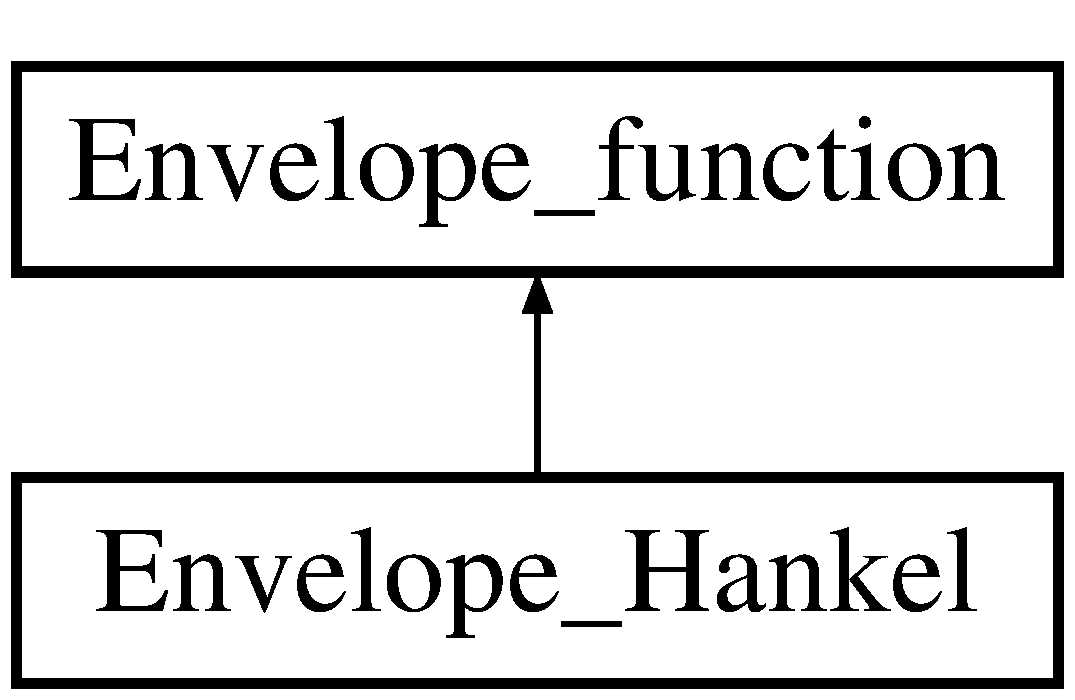
\includegraphics[height=2.000000cm]{classEnvelope__Hankel}
\end{center}
\end{figure}
\subsection*{Public Member Functions}
\begin{DoxyCompactItemize}
\item 
\mbox{\Hypertarget{classEnvelope__Hankel_a1b95e93f11401450c57a047f0979acc8}\label{classEnvelope__Hankel_a1b95e93f11401450c57a047f0979acc8}} 
double {\bfseries barred\+\_\+fun} (double x)
\end{DoxyCompactItemize}
\subsection*{Additional Inherited Members}


The documentation for this class was generated from the following files\+:\begin{DoxyCompactItemize}
\item 
envelope\+\_\+fun.\+h\item 
envelope\+\_\+fun.\+cpp\end{DoxyCompactItemize}

\hypertarget{classEnvelope__Neumann}{}\doxysection{Envelope\+\_\+\+Neumann Class Reference}
\label{classEnvelope__Neumann}\index{Envelope\_Neumann@{Envelope\_Neumann}}
Inheritance diagram for Envelope\+\_\+\+Neumann\+:\begin{figure}[H]
\begin{center}
\leavevmode
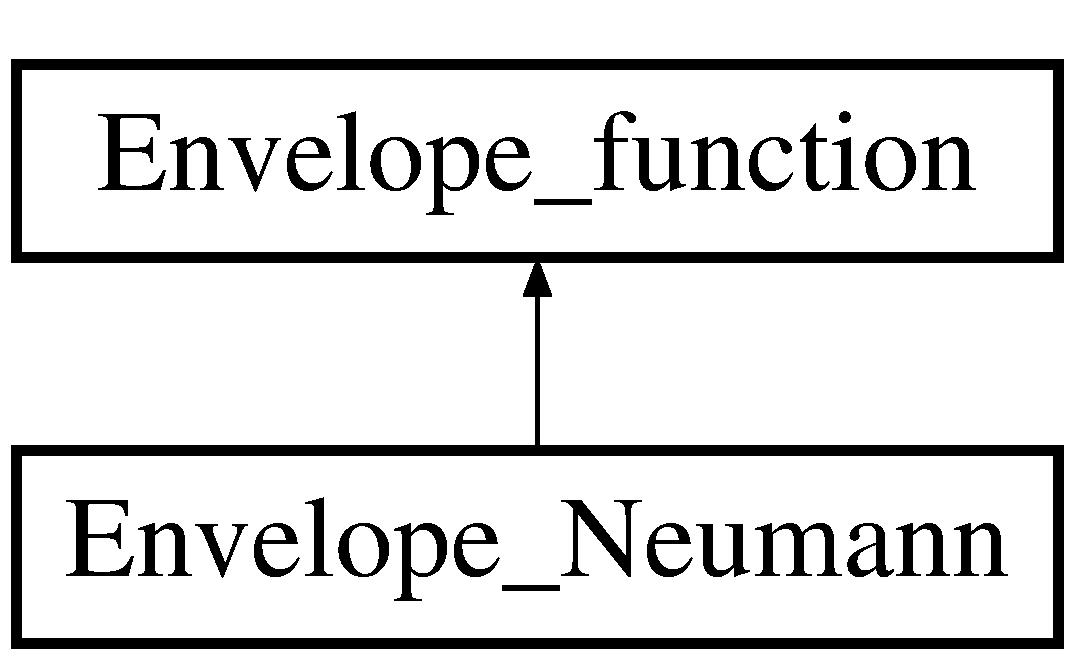
\includegraphics[height=2.000000cm]{classEnvelope__Neumann}
\end{center}
\end{figure}
\doxysubsection*{Public Member Functions}
\begin{DoxyCompactItemize}
\item 
\mbox{\Hypertarget{classEnvelope__Neumann_a1e425fe26f01f06a5ac957a389de4275}\label{classEnvelope__Neumann_a1e425fe26f01f06a5ac957a389de4275}} 
{\bfseries Envelope\+\_\+\+Neumann} (\mbox{\hyperlink{structlm}{lm}} l\+\_\+n, double kappa\+\_\+n)
\item 
\mbox{\Hypertarget{classEnvelope__Neumann_ae01e38e0d0ea4cd19e5942ea669c56b9}\label{classEnvelope__Neumann_ae01e38e0d0ea4cd19e5942ea669c56b9}} 
double {\bfseries barred\+\_\+fun} (const double x) const override
\item 
\mbox{\Hypertarget{classEnvelope__function_a21a876fdc33d23725bdb25990d3f6e6a}\label{classEnvelope__function_a21a876fdc33d23725bdb25990d3f6e6a}} 
double {\bfseries operator()} (const G\+S\+L\+::\+Vector r)
\item 
\mbox{\Hypertarget{classEnvelope__function_a85cd53700d4090e4c0f6dc2e67d7bb42}\label{classEnvelope__function_a85cd53700d4090e4c0f6dc2e67d7bb42}} 
double {\bfseries kappa} () const
\item 
\mbox{\Hypertarget{classEnvelope__function_a94d64257a361bdbf28e2dd525346ceb7}\label{classEnvelope__function_a94d64257a361bdbf28e2dd525346ceb7}} 
double \& {\bfseries kappa} ()
\item 
\mbox{\Hypertarget{classEnvelope__function_a44ac505a0bc963b230a94c0b25d1a61f}\label{classEnvelope__function_a44ac505a0bc963b230a94c0b25d1a61f}} 
\mbox{\hyperlink{structlm}{lm}} {\bfseries l} () const
\item 
\mbox{\Hypertarget{classEnvelope__function_a5caa2943467fe3e75bf8047ef062f196}\label{classEnvelope__function_a5caa2943467fe3e75bf8047ef062f196}} 
\mbox{\hyperlink{structlm}{lm}} \& {\bfseries l} ()
\end{DoxyCompactItemize}
\doxysubsection*{Protected Attributes}
\begin{DoxyCompactItemize}
\item 
\mbox{\Hypertarget{classEnvelope__function_a41518f3ca4477df62028318dd6c88f86}\label{classEnvelope__function_a41518f3ca4477df62028318dd6c88f86}} 
\mbox{\hyperlink{structlm}{lm}} {\bfseries l\+\_\+m}
\item 
\mbox{\Hypertarget{classEnvelope__function_a14925f5c7ac21806a89fd2b7049d47ed}\label{classEnvelope__function_a14925f5c7ac21806a89fd2b7049d47ed}} 
double {\bfseries kappa\+\_\+m}
\end{DoxyCompactItemize}


The documentation for this class was generated from the following file\+:\begin{DoxyCompactItemize}
\item 
envelope\+\_\+fun.\+h\end{DoxyCompactItemize}

\hypertarget{classEwald__integral}{}\section{Ewald\+\_\+integral Class Reference}
\label{classEwald__integral}\index{Ewald\+\_\+integral@{Ewald\+\_\+integral}}


{\ttfamily \#include $<$ewald\+\_\+int.\+h$>$}

\subsection*{Public Member Functions}
\begin{DoxyCompactItemize}
\item 
\mbox{\Hypertarget{classEwald__integral_a81b6312a37021cf8e9a45e417a2c3143}\label{classEwald__integral_a81b6312a37021cf8e9a45e417a2c3143}} 
void \hyperlink{classEwald__integral_a81b6312a37021cf8e9a45e417a2c3143}{set\+\_\+ewald\+\_\+param} (double eta)
\begin{DoxyCompactList}\small\item\em Set the Ewald parameter. \end{DoxyCompactList}\item 
\mbox{\Hypertarget{classEwald__integral_a61619cc2dbdb9cada4552128277aa390}\label{classEwald__integral_a61619cc2dbdb9cada4552128277aa390}} 
void \hyperlink{classEwald__integral_a61619cc2dbdb9cada4552128277aa390}{set\+\_\+kappa} (double kappa)
\begin{DoxyCompactList}\small\item\em Set energy parameter. \end{DoxyCompactList}\item 
\mbox{\Hypertarget{classEwald__integral_acb4f3774a2b38c549791d89aa2040143}\label{classEwald__integral_acb4f3774a2b38c549791d89aa2040143}} 
double {\bfseries ewald\+\_\+int} (\hyperlink{structlm}{lm} l, double r)
\item 
\mbox{\Hypertarget{classEwald__integral_adb1795037f6bfbb41a01f15be2ad27b4}\label{classEwald__integral_adb1795037f6bfbb41a01f15be2ad27b4}} 
double {\bfseries comp\+\_\+ewald\+\_\+int} (\hyperlink{structlm}{lm} l, double r)
\item 
\mbox{\Hypertarget{classEwald__integral_ad3f3f659c22073f76bb1262e47e847fd}\label{classEwald__integral_ad3f3f659c22073f76bb1262e47e847fd}} 
std\+::vector$<$ double $>$ \hyperlink{classEwald__integral_ad3f3f659c22073f76bb1262e47e847fd}{evaluate} (\hyperlink{structlm}{lm} l, \hyperlink{classLogarithmic__mesh}{Logarithmic\+\_\+mesh} \&mesh)
\begin{DoxyCompactList}\small\item\em Calculate the Ewald integral for angular quantum number (l.\+l, l.\+m) and evaluate it on every point in the mesh. \end{DoxyCompactList}\item 
\mbox{\Hypertarget{classEwald__integral_a6cba9e9c66347c0321cd55487304d25a}\label{classEwald__integral_a6cba9e9c66347c0321cd55487304d25a}} 
std\+::vector$<$ double $>$ \hyperlink{classEwald__integral_a6cba9e9c66347c0321cd55487304d25a}{evaluate\+\_\+comp} (\hyperlink{structlm}{lm} l, \hyperlink{classLogarithmic__mesh}{Logarithmic\+\_\+mesh} \&mesh)
\begin{DoxyCompactList}\small\item\em Calculate the complementary Ewald integral for angular quantum number (l.\+l, l.\+m) and evaluate it on every point in the mesh. \end{DoxyCompactList}\item 
\mbox{\Hypertarget{classEwald__integral_acb4f3774a2b38c549791d89aa2040143}\label{classEwald__integral_acb4f3774a2b38c549791d89aa2040143}} 
double {\bfseries ewald\+\_\+int} (\hyperlink{structlm}{lm} l, double r)
\item 
\mbox{\Hypertarget{classEwald__integral_adb1795037f6bfbb41a01f15be2ad27b4}\label{classEwald__integral_adb1795037f6bfbb41a01f15be2ad27b4}} 
double {\bfseries comp\+\_\+ewald\+\_\+int} (\hyperlink{structlm}{lm} l, double r)
\end{DoxyCompactItemize}


\subsection{Detailed Description}
A class for the integral representation of Hankel functions~\newline
Contains\+:~\newline
{\bfseries ewald\+\_\+param} -\/ Parameter separating long range part from short range one~\newline
{\bfseries kappa} -\/ Energy parameter used (usually kappa$^\wedge$2 = -\/0.\+015)~\newline
{\bfseries h} -\/ 

The documentation for this class was generated from the following files\+:\begin{DoxyCompactItemize}
\item 
ewald\+\_\+int.\+h\item 
ewald\+\_\+int.\+cpp\end{DoxyCompactItemize}

\hypertarget{classHankel__function}{}\doxysection{Hankel\+\_\+function Class Reference}
\label{classHankel__function}\index{Hankel\_function@{Hankel\_function}}
Inheritance diagram for Hankel\+\_\+function\+:\begin{figure}[H]
\begin{center}
\leavevmode
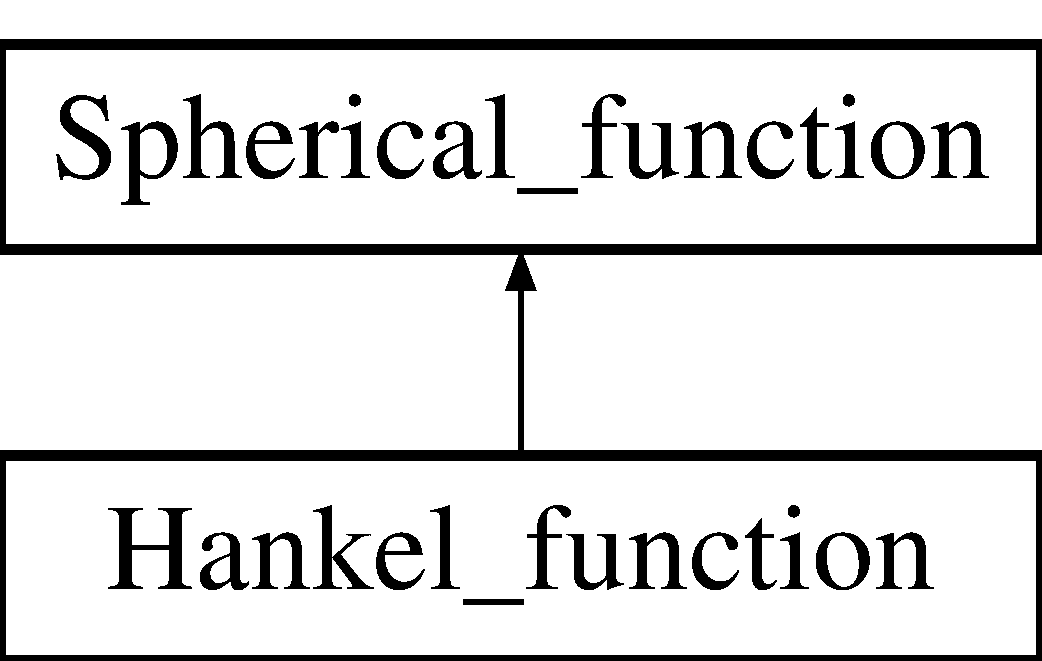
\includegraphics[height=3.000000cm]{classHankel__function}
\end{center}
\end{figure}
\doxysubsection*{Public Member Functions}
\begin{DoxyCompactItemize}
\item 
\mbox{\Hypertarget{classHankel__function_a80a7a0145eb1e3e39b5d290244184d66}\label{classHankel__function_a80a7a0145eb1e3e39b5d290244184d66}} 
{\bfseries Hankel\+\_\+function} (const \mbox{\hyperlink{structlm}{lm}} l\+\_\+n)
\item 
\mbox{\Hypertarget{classHankel__function_af8df068125dfeb7a44b4c9012aee6cc9}\label{classHankel__function_af8df068125dfeb7a44b4c9012aee6cc9}} 
double {\bfseries operator()} (const double x) const override
\item 
\mbox{\Hypertarget{classSpherical__function_a08264bc2e2a8310d8aa0ed496d721ebc}\label{classSpherical__function_a08264bc2e2a8310d8aa0ed496d721ebc}} 
void {\bfseries set\+\_\+l} (const \mbox{\hyperlink{structlm}{lm}} l\+\_\+n)
\item 
\mbox{\Hypertarget{classSpherical__function_aa4290f727726c4544d37680df9b10d3f}\label{classSpherical__function_aa4290f727726c4544d37680df9b10d3f}} 
\mbox{\hyperlink{structlm}{lm}} {\bfseries l} () const
\end{DoxyCompactItemize}
\doxysubsection*{Protected Attributes}
\begin{DoxyCompactItemize}
\item 
\mbox{\Hypertarget{classSpherical__function_a68bc3c4a536d458d6b0432d7a48ed282}\label{classSpherical__function_a68bc3c4a536d458d6b0432d7a48ed282}} 
\mbox{\hyperlink{structlm}{lm}} {\bfseries l\+\_\+m}
\end{DoxyCompactItemize}


The documentation for this class was generated from the following file\+:\begin{DoxyCompactItemize}
\item 
spherical\+\_\+fun.\+h\end{DoxyCompactItemize}

\hypertarget{structstd_1_1hash_3_01Augmented__Bessel_01_4}{}\section{std\+:\+:hash$<$ Augmented\+\_\+\+Bessel $>$ Struct Template Reference}
\label{structstd_1_1hash_3_01Augmented__Bessel_01_4}\index{std\+::hash$<$ Augmented\+\_\+\+Bessel $>$@{std\+::hash$<$ Augmented\+\_\+\+Bessel $>$}}
\subsection*{Public Member Functions}
\begin{DoxyCompactItemize}
\item 
\mbox{\Hypertarget{structstd_1_1hash_3_01Augmented__Bessel_01_4_a81662182d4729c33627b6dbd13797962}\label{structstd_1_1hash_3_01Augmented__Bessel_01_4_a81662182d4729c33627b6dbd13797962}} 
size\+\_\+t {\bfseries operator()} (const \hyperlink{classAugmented__Bessel}{Augmented\+\_\+\+Bessel} \&f) const
\end{DoxyCompactItemize}


The documentation for this struct was generated from the following file\+:\begin{DoxyCompactItemize}
\item 
augmented\+\_\+fun.\+h\end{DoxyCompactItemize}

\hypertarget{structstd_1_1hash_3_01GSL_1_1Vector_01_4}{}\section{std\+:\+:hash$<$ G\+SL\+:\+:Vector $>$ Struct Template Reference}
\label{structstd_1_1hash_3_01GSL_1_1Vector_01_4}\index{std\+::hash$<$ G\+S\+L\+::\+Vector $>$@{std\+::hash$<$ G\+S\+L\+::\+Vector $>$}}
\subsection*{Public Member Functions}
\begin{DoxyCompactItemize}
\item 
\mbox{\Hypertarget{structstd_1_1hash_3_01GSL_1_1Vector_01_4_ad0db7e8b7d16c146e5a738c1e034b762}\label{structstd_1_1hash_3_01GSL_1_1Vector_01_4_ad0db7e8b7d16c146e5a738c1e034b762}} 
size\+\_\+t {\bfseries operator()} (const G\+S\+L\+::\+Vector \&v) const
\end{DoxyCompactItemize}


The documentation for this struct was generated from the following file\+:\begin{DoxyCompactItemize}
\item 
crystal.\+cpp\end{DoxyCompactItemize}

\hypertarget{classLattice}{}\section{Lattice Class Reference}
\label{classLattice}\index{Lattice@{Lattice}}


{\ttfamily \#include $<$lattice.\+h$>$}

\subsection*{Public Member Functions}
\begin{DoxyCompactItemize}
\item 
\mbox{\Hypertarget{classLattice_abb8611ee57bcfd97a471e81451cdf8a7}\label{classLattice_abb8611ee57bcfd97a471e81451cdf8a7}} 
{\bfseries Lattice} (G\+S\+L\+::\+Vector \&a, G\+S\+L\+::\+Vector \&b, G\+S\+L\+::\+Vector \&c)
\item 
\mbox{\Hypertarget{classLattice_adfd826f48fcc01b337477dd54eb39a73}\label{classLattice_adfd826f48fcc01b337477dd54eb39a73}} 
{\bfseries Lattice} (const G\+S\+L\+::\+Vector \&a, const G\+S\+L\+::\+Vector \&b, const G\+S\+L\+::\+Vector \&c)
\end{DoxyCompactItemize}
\subsection*{Public Attributes}
\begin{DoxyCompactItemize}
\item 
\mbox{\Hypertarget{classLattice_adc1824ce4a46c80439562083583462e6}\label{classLattice_adc1824ce4a46c80439562083583462e6}} 
G\+S\+L\+::\+Matrix {\bfseries lat}
\item 
\mbox{\Hypertarget{classLattice_adf55e46c0238b3585962ebd52264f326}\label{classLattice_adf55e46c0238b3585962ebd52264f326}} 
G\+S\+L\+::\+Matrix {\bfseries r\+\_\+lat}
\item 
\mbox{\Hypertarget{classLattice_aca4e74198ee01bbe9e1bb70adc98d904}\label{classLattice_aca4e74198ee01bbe9e1bb70adc98d904}} 
double {\bfseries scale}
\item 
\mbox{\Hypertarget{classLattice_a907782dea80f8e3657afc2bcad10a837}\label{classLattice_a907782dea80f8e3657afc2bcad10a837}} 
double {\bfseries volume}
\item 
\mbox{\Hypertarget{classLattice_a2593512591334fbe6857f2fa6e536469}\label{classLattice_a2593512591334fbe6857f2fa6e536469}} 
double {\bfseries bz\+\_\+volume}
\end{DoxyCompactItemize}


\subsection{Detailed Description}
A class used to represent lattices, e.\+g. Bravais lattices useful in describing crystals.~\newline
 Contains\+:~\newline
 {\bfseries lat} -\/ G\+S\+L\+::\+Matrix constructed from the three lattice vectors (row major). ~\newline
 {\bfseries r\+\_\+lat} -\/ G\+S\+L\+::\+Matrix constructed from the three reciprocal lattice vectors (row major).~\newline
 {\bfseries scale} -\/ Scale factor to multiply each lattice vector with.~\newline
 {\bfseries volume} -\/ Volume of the unit cell.~\newline
 {\bfseries bz\+\_\+volume} -\/ Volume of the first Brillouin zone.~\newline


The documentation for this class was generated from the following files\+:\begin{DoxyCompactItemize}
\item 
lattice.\+h\item 
lattice.\+cpp\end{DoxyCompactItemize}

\hypertarget{structlm}{}\section{lm Struct Reference}
\label{structlm}\index{lm@{lm}}


{\ttfamily \#include $<$utils.\+h$>$}

\subsection*{Public Attributes}
\begin{DoxyCompactItemize}
\item 
\mbox{\Hypertarget{structlm_a7b9984283d01c4d8e720fea5412bd498}\label{structlm_a7b9984283d01c4d8e720fea5412bd498}} 
int {\bfseries l}
\item 
\mbox{\Hypertarget{structlm_a2884b87159292304e4ee24c9e5c8c507}\label{structlm_a2884b87159292304e4ee24c9e5c8c507}} 
int {\bfseries m}
\end{DoxyCompactItemize}


\subsection{Detailed Description}
Data type for representing combined orbital and magnetic quantum numbers.~\newline


The documentation for this struct was generated from the following file\+:\begin{DoxyCompactItemize}
\item 
utils.\+h\end{DoxyCompactItemize}

\hypertarget{classLogarithmic__mesh}{}\section{Logarithmic\+\_\+mesh Class Reference}
\label{classLogarithmic__mesh}\index{Logarithmic\+\_\+mesh@{Logarithmic\+\_\+mesh}}


{\ttfamily \#include $<$log\+\_\+mesh.\+h$>$}

\subsection*{Public Member Functions}
\begin{DoxyCompactItemize}
\item 
\mbox{\Hypertarget{classLogarithmic__mesh_ad9294c2de86a826584489ff2b7dd3963}\label{classLogarithmic__mesh_ad9294c2de86a826584489ff2b7dd3963}} 
{\bfseries Logarithmic\+\_\+mesh} (double radius, unsigned int num\+\_\+points)
\item 
\mbox{\Hypertarget{classLogarithmic__mesh_a3c394001d97d86907ef5e9f61dd680ca}\label{classLogarithmic__mesh_a3c394001d97d86907ef5e9f61dd680ca}} 
{\bfseries Logarithmic\+\_\+mesh} (double A, double radius, unsigned int num\+\_\+points)
\item 
\mbox{\Hypertarget{classLogarithmic__mesh_aa832cd52424296e6d519313558eb3132}\label{classLogarithmic__mesh_aa832cd52424296e6d519313558eb3132}} 
double {\bfseries radial\+\_\+integral} (std\+::vector$<$ double $>$ f)
\end{DoxyCompactItemize}
\subsection*{Public Attributes}
\begin{DoxyCompactItemize}
\item 
\mbox{\Hypertarget{classLogarithmic__mesh_a78084fd600b2ded00b34b5b8f705f5a4}\label{classLogarithmic__mesh_a78084fd600b2ded00b34b5b8f705f5a4}} 
std\+::vector$<$ double $>$ {\bfseries r}
\item 
\mbox{\Hypertarget{classLogarithmic__mesh_a297cb20a293a3ba26250b55fad36f88b}\label{classLogarithmic__mesh_a297cb20a293a3ba26250b55fad36f88b}} 
std\+::vector$<$ double $>$ {\bfseries r2}
\item 
\mbox{\Hypertarget{classLogarithmic__mesh_af7e95466d3c76af1c34c6c014569906c}\label{classLogarithmic__mesh_af7e95466d3c76af1c34c6c014569906c}} 
std\+::vector$<$ double $>$ {\bfseries drx}
\item 
\mbox{\Hypertarget{classLogarithmic__mesh_a879e08e3f2ccc6fe2933110bbe649152}\label{classLogarithmic__mesh_a879e08e3f2ccc6fe2933110bbe649152}} 
double {\bfseries A}
\end{DoxyCompactItemize}


\subsection{Detailed Description}
A class for representing logarithmic meshes~\newline
Contains\+:~\newline
{\bfseries B} -\/ Parameter determining shape of mesh, calculated from {\bfseries num\+\_\+points} and {\bfseries A}~\newline
{\bfseries r} -\/ r-\/values contained in mesh~\newline
{\bfseries r2} -\/ r$^\wedge$2-\/values contained in mesh~\newline
{\bfseries drx} -\/ Derivative dr/dx evaluated in mesh~\newline
{\bfseries A} -\/ Parameter controlling spacing between points in mesh~\newline


The documentation for this class was generated from the following files\+:\begin{DoxyCompactItemize}
\item 
log\+\_\+mesh.\+h\item 
log\+\_\+mesh.\+cpp\end{DoxyCompactItemize}

\hypertarget{classNeumann__function}{}\section{Neumann\+\_\+function Class Reference}
\label{classNeumann__function}\index{Neumann\+\_\+function@{Neumann\+\_\+function}}
Inheritance diagram for Neumann\+\_\+function\+:\begin{figure}[H]
\begin{center}
\leavevmode
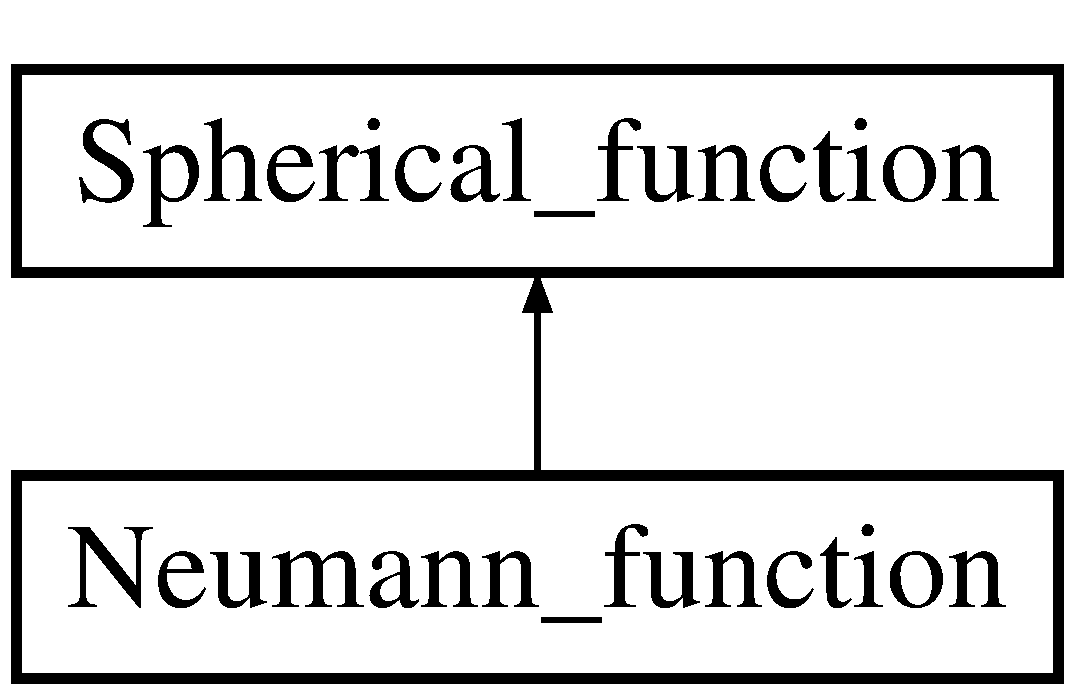
\includegraphics[height=2.000000cm]{classNeumann__function}
\end{center}
\end{figure}
\subsection*{Public Member Functions}
\begin{DoxyCompactItemize}
\item 
\mbox{\Hypertarget{classNeumann__function_aa4aefbe0c19a40d5aa39f4a5d5c23473}\label{classNeumann__function_aa4aefbe0c19a40d5aa39f4a5d5c23473}} 
{\bfseries Neumann\+\_\+function} (const \hyperlink{structlm}{lm} l)
\item 
\mbox{\Hypertarget{classNeumann__function_a423faa23869a1e6c1071ccc8e35a2258}\label{classNeumann__function_a423faa23869a1e6c1071ccc8e35a2258}} 
double {\bfseries operator()} (const double x)
\end{DoxyCompactItemize}
\subsection*{Additional Inherited Members}


The documentation for this class was generated from the following files\+:\begin{DoxyCompactItemize}
\item 
spherical\+\_\+fun.\+h\item 
spherical\+\_\+fun.\+cpp\end{DoxyCompactItemize}

\hypertarget{classNumerov__solver}{}\doxysection{Numerov\+\_\+solver Class Reference}
\label{classNumerov__solver}\index{Numerov\_solver@{Numerov\_solver}}


{\ttfamily \#include $<$numerov\+\_\+solver.\+h$>$}

\doxysubsection*{Public Member Functions}
\begin{DoxyCompactItemize}
\item 
{\footnotesize template$<$class Iter\+\_\+res , class Iter\+\_\+g , class Iter\+\_\+s , class Iter\+\_\+left\+\_\+init , class Iter\+\_\+right\+\_\+init , class T  = double$>$ }\\Iter\+\_\+res \mbox{\hyperlink{classNumerov__solver_a65b9b13d9163fe41de27069f420d8ee3}{solve}} (Iter\+\_\+res res\+\_\+start, Iter\+\_\+res res\+\_\+end, Iter\+\_\+g g\+\_\+start, Iter\+\_\+g g\+\_\+end, Iter\+\_\+s s\+\_\+start, Iter\+\_\+s s\+\_\+end, Iter\+\_\+left\+\_\+init left\+\_\+start, Iter\+\_\+left\+\_\+init left\+\_\+end, Iter\+\_\+right\+\_\+init right\+\_\+start, Iter\+\_\+right\+\_\+init right\+\_\+end, Iter\+\_\+res inv)
\item 
{\footnotesize template$<$class Iter\+\_\+res , class Iter\+\_\+g , class Iter\+\_\+s , class Iter\+\_\+left\+\_\+init , class Iter\+\_\+right\+\_\+init , class T  = double$>$ }\\Iter\+\_\+res \mbox{\hyperlink{classNumerov__solver_ad36887819ca68c3ea9033a065c627c6d}{solve}} (Iter\+\_\+res res\+\_\+start, Iter\+\_\+res res\+\_\+end, Iter\+\_\+g g\+\_\+start, Iter\+\_\+g g\+\_\+end, Iter\+\_\+s s\+\_\+start, Iter\+\_\+s s\+\_\+end, Iter\+\_\+left\+\_\+init left\+\_\+start, Iter\+\_\+left\+\_\+init left\+\_\+end)
\item 
{\footnotesize template$<$class Iter\+\_\+res , class Iter\+\_\+g , class Iter\+\_\+s , class T  = double$>$ }\\int \mbox{\hyperlink{classNumerov__solver_aa1937256e243d0a408cb71928d857713}{derivative\+\_\+diff}} (Iter\+\_\+res res\+\_\+start, Iter\+\_\+g res\+\_\+end, Iter\+\_\+res inv, Iter\+\_\+g g\+\_\+start, Iter\+\_\+s s\+\_\+start, double tol=1e-\/6)
\item 
\mbox{\Hypertarget{classNumerov__solver_aeae9b9ffa364c9e7eb86f5444f839a33}\label{classNumerov__solver_aeae9b9ffa364c9e7eb86f5444f839a33}} 
{\footnotesize template$<$class Iter\+\_\+res $>$ }\\int {\bfseries count\+\_\+nodes} (Iter\+\_\+res start, Iter\+\_\+res end)
\end{DoxyCompactItemize}


\doxysubsection{Detailed Description}
A class for solving differential equations using the Numerov method 

\doxysubsection{Member Function Documentation}
\mbox{\Hypertarget{classNumerov__solver_aa1937256e243d0a408cb71928d857713}\label{classNumerov__solver_aa1937256e243d0a408cb71928d857713}} 
\index{Numerov\_solver@{Numerov\_solver}!derivative\_diff@{derivative\_diff}}
\index{derivative\_diff@{derivative\_diff}!Numerov\_solver@{Numerov\_solver}}
\doxysubsubsection{\texorpdfstring{derivative\_diff()}{derivative\_diff()}}
{\footnotesize\ttfamily template$<$class Iter\+\_\+res , class Iter\+\_\+g , class Iter\+\_\+s , class T  = double$>$ \\
int Numerov\+\_\+solver\+::derivative\+\_\+diff (\begin{DoxyParamCaption}\item[{Iter\+\_\+res}]{res\+\_\+start,  }\item[{Iter\+\_\+g}]{res\+\_\+end,  }\item[{Iter\+\_\+res}]{inv,  }\item[{Iter\+\_\+g}]{g\+\_\+start,  }\item[{Iter\+\_\+s}]{s\+\_\+start,  }\item[{double}]{tol = {\ttfamily 1e-\/6} }\end{DoxyParamCaption})\hspace{0.3cm}{\ttfamily [inline]}}

Use Numerov\textquotesingle{}s algorithm to estimate the difference in derivatives at the matching point. \textbackslash{}t\+\_\+\+\_\+\+Iter\+\_\+res\+\_\+\+\_\+ -\/ iterator to result container (e.\+g. std\+::vector)~\newline
 \textbackslash{}t\+\_\+\+\_\+\+Iter\+\_\+g\+\_\+\+\_\+ -\/ iterator to g container (e.\+g. std\+::vector)~\newline
 \textbackslash{}t\+\_\+\+\_\+\+Iter\+\_\+s\+\_\+\+\_\+ -\/ iterator to s container (e.\+g. std\+::vector)~\newline
 \textbackslash{}t\+\_\+\+\_\+\+T\+\_\+\+\_\+ -\/ Class representing numerical values (e.\+g. double)~\newline
 Input\+:~\newline
 \textbackslash{}t\+\_\+\+\_\+res\+\_\+start\+\_\+\+\_\+ -\/ iterator to the first element in the result container~\newline
 \textbackslash{}t\+\_\+\+\_\+res\+\_\+end\+\_\+\+\_\+ -\/ iterator one step part the last element in the result container~\newline
 \textbackslash{}t\+\_\+\+\_\+inv\+\_\+\+\_\+ -\/ iterator to result at inversion point~\newline
 \textbackslash{}t\+\_\+\+\_\+g\+\_\+start\+\_\+\+\_\+ -\/ iterator to the start of the g container~\newline
 \textbackslash{}t\+\_\+\+\_\+s\+\_\+start\+\_\+\+\_\+ -\/ iterator to the start of the s container~\newline
Returns\+:~\newline
\textbackslash{}t Approximation of sign(y\textquotesingle{}\+\_\+\+R(x\+\_\+inv) -\/ y\textquotesingle{}\+\_\+\+L(x\+\_\+inv)), sign of the difference in derivatives.~\newline
N\+O\+TE \+: The elements of g must be multiplied with the step size squared (h$^\wedge$2). \mbox{\Hypertarget{classNumerov__solver_ad36887819ca68c3ea9033a065c627c6d}\label{classNumerov__solver_ad36887819ca68c3ea9033a065c627c6d}} 
\index{Numerov\_solver@{Numerov\_solver}!solve@{solve}}
\index{solve@{solve}!Numerov\_solver@{Numerov\_solver}}
\doxysubsubsection{\texorpdfstring{solve()}{solve()}\hspace{0.1cm}{\footnotesize\ttfamily [1/2]}}
{\footnotesize\ttfamily template$<$class Iter\+\_\+res , class Iter\+\_\+g , class Iter\+\_\+s , class Iter\+\_\+left\+\_\+init , class Iter\+\_\+right\+\_\+init , class T  = double$>$ \\
Iter\+\_\+res Numerov\+\_\+solver\+::solve (\begin{DoxyParamCaption}\item[{Iter\+\_\+res}]{res\+\_\+start,  }\item[{Iter\+\_\+res}]{res\+\_\+end,  }\item[{Iter\+\_\+g}]{g\+\_\+start,  }\item[{Iter\+\_\+g}]{g\+\_\+end,  }\item[{Iter\+\_\+s}]{s\+\_\+start,  }\item[{Iter\+\_\+s}]{s\+\_\+end,  }\item[{Iter\+\_\+left\+\_\+init}]{left\+\_\+start,  }\item[{Iter\+\_\+left\+\_\+init}]{left\+\_\+end }\end{DoxyParamCaption})\hspace{0.3cm}{\ttfamily [inline]}}

Solve in one direction only. Overloaded version of solve. \mbox{\Hypertarget{classNumerov__solver_a65b9b13d9163fe41de27069f420d8ee3}\label{classNumerov__solver_a65b9b13d9163fe41de27069f420d8ee3}} 
\index{Numerov\_solver@{Numerov\_solver}!solve@{solve}}
\index{solve@{solve}!Numerov\_solver@{Numerov\_solver}}
\doxysubsubsection{\texorpdfstring{solve()}{solve()}\hspace{0.1cm}{\footnotesize\ttfamily [2/2]}}
{\footnotesize\ttfamily template$<$class Iter\+\_\+res , class Iter\+\_\+g , class Iter\+\_\+s , class Iter\+\_\+left\+\_\+init , class Iter\+\_\+right\+\_\+init , class T  = double$>$ \\
Iter\+\_\+res Numerov\+\_\+solver\+::solve (\begin{DoxyParamCaption}\item[{Iter\+\_\+res}]{res\+\_\+start,  }\item[{Iter\+\_\+res}]{res\+\_\+end,  }\item[{Iter\+\_\+g}]{g\+\_\+start,  }\item[{Iter\+\_\+g}]{g\+\_\+end,  }\item[{Iter\+\_\+s}]{s\+\_\+start,  }\item[{Iter\+\_\+s}]{s\+\_\+end,  }\item[{Iter\+\_\+left\+\_\+init}]{left\+\_\+start,  }\item[{Iter\+\_\+left\+\_\+init}]{left\+\_\+end,  }\item[{Iter\+\_\+right\+\_\+init}]{right\+\_\+start,  }\item[{Iter\+\_\+right\+\_\+init}]{right\+\_\+end,  }\item[{Iter\+\_\+res}]{inv }\end{DoxyParamCaption})\hspace{0.3cm}{\ttfamily [inline]}}

Use Numerov\textquotesingle{}s algorithm to solve the differential equation. \textbackslash{}t\+\_\+\+\_\+\+Iter\+\_\+res\+\_\+\+\_\+ -\/ iterator to result container (e.\+g. std\+::vector)~\newline
 \textbackslash{}t\+\_\+\+\_\+\+Iter\+\_\+g\+\_\+\+\_\+ -\/ iterator to g container (e.\+g. std\+::vector)~\newline
 Input\+:~\newline
 \textbackslash{}t\+\_\+\+\_\+res\+\_\+start\+\_\+\+\_\+ -\/ iterator to the first element in the result container~\newline
 \textbackslash{}t\+\_\+\+\_\+res\+\_\+end\+\_\+\+\_\+ -\/ iterator one step part the last element in the result container~\newline
 \textbackslash{}t\+\_\+\+\_\+g\+\_\+start\+\_\+\+\_\+ -\/ iterator to the start of the g container~\newline
 \textbackslash{}t\+\_\+\+\_\+g\+\_\+end\+\_\+\+\_\+ -\/ iterator to one step past the last element of the g container~\newline
 \textbackslash{}t\+\_\+\+\_\+s\+\_\+start\+\_\+\+\_\+ -\/ iterator to the start of the s container~\newline
 \textbackslash{}t\+\_\+\+\_\+s\+\_\+end\+\_\+\+\_\+ -\/ iterator to one step past the last element of the s container~\newline
 \textbackslash{}t\+\_\+\+\_\+left\+\_\+start\+\_\+\+\_\+ -\/ iterator to the start of the container containing the left hand initial conditions~\newline
 \textbackslash{}t\+\_\+\+\_\+left\+\_\+end\+\_\+\+\_\+ -\/ iterator to one step past the last element of the left boundary conditions container~\newline
 \textbackslash{}t\+\_\+\+\_\+right\+\_\+start\+\_\+\+\_\+ -\/ iterator to the start of the container containing the right hand initial conditions~\newline
 \textbackslash{}t\+\_\+\+\_\+right\+\_\+end\+\_\+\+\_\+ -\/ iterator to one step past the last element of the right boundary conditions container~\newline
Returns\+:~\newline
\textbackslash{}t Iterator to the matching point.~\newline
N\+O\+TE \+: The elements of g must be multiplied with the step size squared (h$^\wedge$2). 

The documentation for this class was generated from the following file\+:\begin{DoxyCompactItemize}
\item 
numerov\+\_\+solver.\+h\end{DoxyCompactItemize}

\hypertarget{classPotential}{}\doxysection{Potential Class Reference}
\label{classPotential}\index{Potential@{Potential}}
Inheritance diagram for Potential\+:\begin{figure}[H]
\begin{center}
\leavevmode
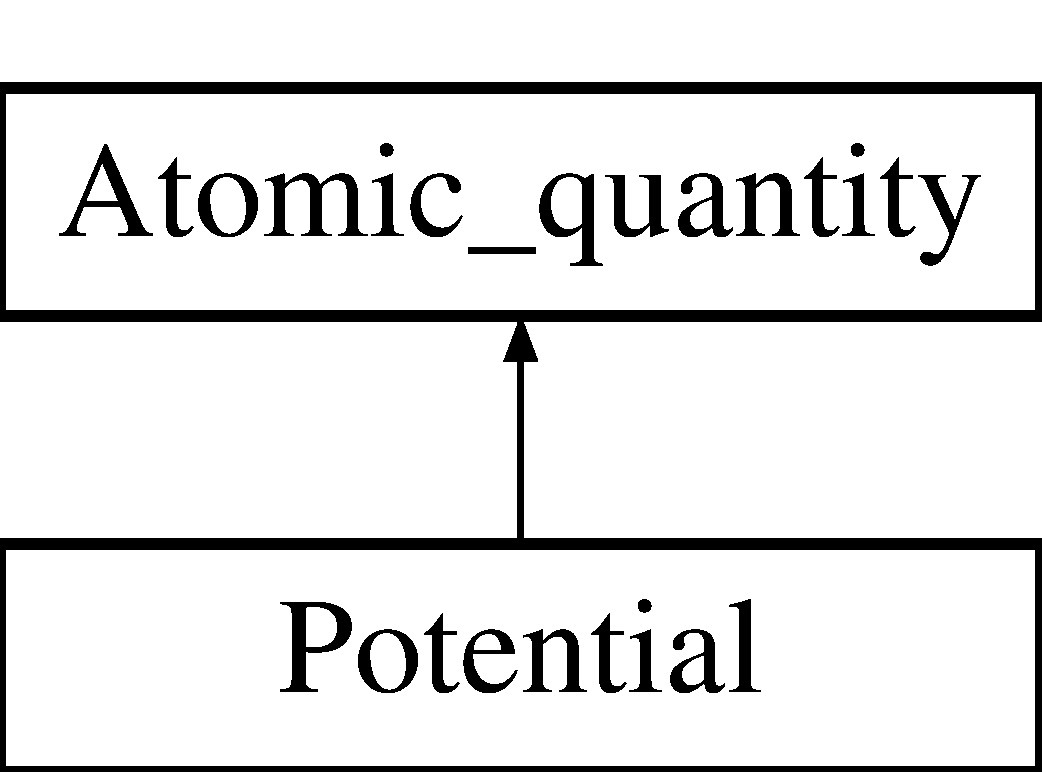
\includegraphics[height=2.000000cm]{classPotential}
\end{center}
\end{figure}
\doxysubsection*{Public Member Functions}
\begin{DoxyCompactItemize}
\item 
\mbox{\Hypertarget{classPotential_afff42668a768c6309d94d069ae34824d}\label{classPotential_afff42668a768c6309d94d069ae34824d}} 
void {\bfseries initial\+\_\+pot} (double vol)
\item 
\mbox{\Hypertarget{classPotential_a2e233e4d4bec88f4961cb1b2e2b81890}\label{classPotential_a2e233e4d4bec88f4961cb1b2e2b81890}} 
double {\bfseries M\+T0} ()
\item 
\mbox{\Hypertarget{classPotential_a688eff314106f0421254da2c77288d00}\label{classPotential_a688eff314106f0421254da2c77288d00}} 
{\bfseries Potential} (const \mbox{\hyperlink{classCrystal__t}{Crystal\+\_\+t}}$<$ 3, \mbox{\hyperlink{classAtom}{Atom}} $>$ \&cryst, const std\+::vector$<$ \mbox{\hyperlink{classLogarithmic__mesh}{Logarithmic\+\_\+mesh}} $>$ \&at\+\_\+meshes, std\+::function$<$ double(const size\+\_\+t Z, const double r)$>$ atomic\+\_\+potential=\mbox{[}$\,$\mbox{]}(const size\+\_\+t Z, const double r)\{ return -\/2.$\ast$static\+\_\+cast$<$ double $>$(Z)/r;\})
\item 
\mbox{\Hypertarget{classPotential_a6a6eca1dc9b32494f6189404e503eb38}\label{classPotential_a6a6eca1dc9b32494f6189404e503eb38}} 
void {\bfseries set\+\_\+xc\+\_\+fun} (X\+C\+\_\+\+F\+UN xc\+\_\+func)
\item 
\mbox{\Hypertarget{classAtomic__quantity_a5bd9055fdf94e57e54a355d5aa818b6c}\label{classAtomic__quantity_a5bd9055fdf94e57e54a355d5aa818b6c}} 
double {\bfseries operator()} (const G\+S\+L\+::\+Vector \&r)
\item 
\mbox{\Hypertarget{classAtomic__quantity_adfdeab2507a0b975643b53b1df2319b1}\label{classAtomic__quantity_adfdeab2507a0b975643b53b1df2319b1}} 
std\+::vector$<$ double $>$ \& {\bfseries sphere} (const size\+\_\+t i)
\end{DoxyCompactItemize}
\doxysubsection*{Public Attributes}
\begin{DoxyCompactItemize}
\item 
\mbox{\Hypertarget{classPotential_a6a99f6673af280be1d6eb3d6e0a963bb}\label{classPotential_a6a99f6673af280be1d6eb3d6e0a963bb}} 
\mbox{\hyperlink{classXc__func}{Xc\+\_\+func}} {\bfseries xc\+\_\+fun}
\end{DoxyCompactItemize}
\doxysubsection*{Protected Attributes}
\begin{DoxyCompactItemize}
\item 
\mbox{\Hypertarget{classAtomic__quantity_a0fb317241d287bde4bbee6cade84a45f}\label{classAtomic__quantity_a0fb317241d287bde4bbee6cade84a45f}} 
const \mbox{\hyperlink{classCrystal__t}{Crystal\+\_\+t}}$<$ 3, \mbox{\hyperlink{classAtom}{Atom}} $>$ \& {\bfseries cr}
\item 
\mbox{\Hypertarget{classAtomic__quantity_a38619ec6589df0672464f3512243c13f}\label{classAtomic__quantity_a38619ec6589df0672464f3512243c13f}} 
const std\+::vector$<$ \mbox{\hyperlink{classLogarithmic__mesh}{Logarithmic\+\_\+mesh}} $>$ \& {\bfseries at\+\_\+meshes}
\item 
\mbox{\Hypertarget{classAtomic__quantity_a69f4c5e435c8c32883528b7cf2099616}\label{classAtomic__quantity_a69f4c5e435c8c32883528b7cf2099616}} 
std\+::vector$<$ std\+::vector$<$ double $>$ $>$ {\bfseries val}
\end{DoxyCompactItemize}


The documentation for this class was generated from the following file\+:\begin{DoxyCompactItemize}
\item 
atomic\+\_\+quantity.\+h\end{DoxyCompactItemize}

\hypertarget{classSpherical__function}{}\doxysection{Spherical\+\_\+function Class Reference}
\label{classSpherical__function}\index{Spherical\_function@{Spherical\_function}}
Inheritance diagram for Spherical\+\_\+function\+:\begin{figure}[H]
\begin{center}
\leavevmode
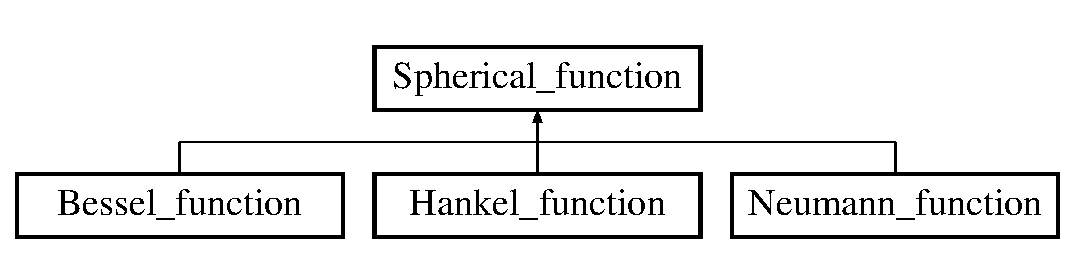
\includegraphics[height=3.000000cm]{classSpherical__function}
\end{center}
\end{figure}
\doxysubsection*{Public Member Functions}
\begin{DoxyCompactItemize}
\item 
\mbox{\Hypertarget{classSpherical__function_aaf2d510641ef38d856f97faba997fb8c}\label{classSpherical__function_aaf2d510641ef38d856f97faba997fb8c}} 
{\bfseries Spherical\+\_\+function} (const \mbox{\hyperlink{structlm}{lm}} l\+\_\+n)
\item 
\mbox{\Hypertarget{classSpherical__function_a8ce17f2efebc998837dbf49a270b0eb9}\label{classSpherical__function_a8ce17f2efebc998837dbf49a270b0eb9}} 
{\bfseries Spherical\+\_\+function} (const \mbox{\hyperlink{classSpherical__function}{Spherical\+\_\+function}} \&f)=default
\item 
\mbox{\Hypertarget{classSpherical__function_a25f1ce863baeabf7707fc6722c6cb701}\label{classSpherical__function_a25f1ce863baeabf7707fc6722c6cb701}} 
{\bfseries Spherical\+\_\+function} (\mbox{\hyperlink{classSpherical__function}{Spherical\+\_\+function}} \&\&f)=default
\item 
\mbox{\Hypertarget{classSpherical__function_aa3d57bcf0f68bfc1736630ed8103e290}\label{classSpherical__function_aa3d57bcf0f68bfc1736630ed8103e290}} 
\mbox{\hyperlink{classSpherical__function}{Spherical\+\_\+function}} \& {\bfseries operator=} (const \mbox{\hyperlink{classSpherical__function}{Spherical\+\_\+function}} \&f)=default
\item 
\mbox{\Hypertarget{classSpherical__function_a542d453e04488bec25693b1bde4dc34e}\label{classSpherical__function_a542d453e04488bec25693b1bde4dc34e}} 
\mbox{\hyperlink{classSpherical__function}{Spherical\+\_\+function}} \& {\bfseries operator=} (\mbox{\hyperlink{classSpherical__function}{Spherical\+\_\+function}} \&\&f)=default
\item 
\mbox{\Hypertarget{classSpherical__function_aa8af0f3183f7725ee1f70ce7644ed822}\label{classSpherical__function_aa8af0f3183f7725ee1f70ce7644ed822}} 
virtual double {\bfseries operator()} (const double x) const
\item 
\mbox{\Hypertarget{classSpherical__function_a08264bc2e2a8310d8aa0ed496d721ebc}\label{classSpherical__function_a08264bc2e2a8310d8aa0ed496d721ebc}} 
void {\bfseries set\+\_\+l} (const \mbox{\hyperlink{structlm}{lm}} l\+\_\+n)
\item 
\mbox{\Hypertarget{classSpherical__function_aa4290f727726c4544d37680df9b10d3f}\label{classSpherical__function_aa4290f727726c4544d37680df9b10d3f}} 
\mbox{\hyperlink{structlm}{lm}} {\bfseries l} () const
\end{DoxyCompactItemize}
\doxysubsection*{Protected Attributes}
\begin{DoxyCompactItemize}
\item 
\mbox{\Hypertarget{classSpherical__function_a68bc3c4a536d458d6b0432d7a48ed282}\label{classSpherical__function_a68bc3c4a536d458d6b0432d7a48ed282}} 
\mbox{\hyperlink{structlm}{lm}} {\bfseries l\+\_\+m}
\end{DoxyCompactItemize}


The documentation for this class was generated from the following file\+:\begin{DoxyCompactItemize}
\item 
spherical\+\_\+fun.\+h\end{DoxyCompactItemize}

\hypertarget{classStructure__constant}{}\section{Structure\+\_\+constant Class Reference}
\label{classStructure__constant}\index{Structure\+\_\+constant@{Structure\+\_\+constant}}


{\ttfamily \#include $<$structure\+\_\+const.\+h$>$}

\subsection*{Public Member Functions}
\begin{DoxyCompactItemize}
\item 
\mbox{\Hypertarget{classStructure__constant_a3ec54c7f725377c9a0a1c070150ca8ac}\label{classStructure__constant_a3ec54c7f725377c9a0a1c070150ca8ac}} 
{\bfseries Structure\+\_\+constant} (int l\+\_\+low, int l\+\_\+int, double kappa, \hyperlink{structlm}{lm} l1, \hyperlink{structlm}{lm} l2, G\+S\+L\+::\+Vector \&r)
\item 
\mbox{\Hypertarget{classStructure__constant_a0738527824a89745ccfbf5c3574591e2}\label{classStructure__constant_a0738527824a89745ccfbf5c3574591e2}} 
{\bfseries Structure\+\_\+constant} (int l\+\_\+low, int l\+\_\+int, \hyperlink{structlm}{lm} l1, \hyperlink{structlm}{lm} l2, G\+S\+L\+::\+Vector \&r)
\item 
\mbox{\Hypertarget{classStructure__constant_a10517723cc79639846ccbdb08f3c0c3f}\label{classStructure__constant_a10517723cc79639846ccbdb08f3c0c3f}} 
{\bfseries Structure\+\_\+constant} (int l\+\_\+low, \hyperlink{structlm}{lm} l1, \hyperlink{structlm}{lm} l2, G\+S\+L\+::\+Vector \&r)
\item 
\mbox{\Hypertarget{classStructure__constant_aed388efe9aed5398b5a61ee57b269d2f}\label{classStructure__constant_aed388efe9aed5398b5a61ee57b269d2f}} 
{\bfseries Structure\+\_\+constant} (\hyperlink{structlm}{lm} l1, \hyperlink{structlm}{lm} l2, G\+S\+L\+::\+Vector \&r)
\end{DoxyCompactItemize}
\subsection*{Public Attributes}
\begin{DoxyCompactItemize}
\item 
\mbox{\Hypertarget{classStructure__constant_a1155f4863b1c995729abce2c93697595}\label{classStructure__constant_a1155f4863b1c995729abce2c93697595}} 
double {\bfseries val}
\item 
\mbox{\Hypertarget{classStructure__constant_ac361c2fe9165b85c4ffe4d72d323524a}\label{classStructure__constant_ac361c2fe9165b85c4ffe4d72d323524a}} 
double {\bfseries dk\+\_\+val}
\end{DoxyCompactItemize}
\subsection*{Friends}
\begin{DoxyCompactItemize}
\item 
\mbox{\Hypertarget{classStructure__constant_af633c21967d44869e756f9f33428cb6a}\label{classStructure__constant_af633c21967d44869e756f9f33428cb6a}} 
std\+::ostream \& {\bfseries operator$<$$<$} (std\+::ostream \&, const \hyperlink{classStructure__constant}{Structure\+\_\+constant} \&)
\end{DoxyCompactItemize}


\subsection{Detailed Description}
A class for representing structure constants~\newline
Contains\+:~\newline
{\bfseries l\+\_\+int} -\/ Maximum orbital angular momentum to be included for Bessel expansions~\newline
 {\bfseries l\+\_\+low} -\/ Maximumm orbital angular momentum to be included for Hankel expansions~\newline
 {\bfseries l1}, {\bfseries l2} -\/ Orbital angular momenta to couple via the structure constant~\newline
{\bfseries kappa} -\/ Energy parameter used (usually kappa$^\wedge$2 = -\/0.\+015)~\newline
{\bfseries r} -\/ Position of atom~\newline
{\bfseries val} -\/ Value of the structure constant~\newline
{\bfseries dk\+\_\+val} -\/ Value of energy derivative of the structure constant~\newline


The documentation for this class was generated from the following files\+:\begin{DoxyCompactItemize}
\item 
structure\+\_\+const.\+h\item 
structure\+\_\+const.\+cpp\end{DoxyCompactItemize}

\hypertarget{classXc__func}{}\section{Xc\+\_\+func Class Reference}
\label{classXc__func}\index{Xc\+\_\+func@{Xc\+\_\+func}}
\subsection*{Public Member Functions}
\begin{DoxyCompactItemize}
\item 
\mbox{\Hypertarget{classXc__func_af1ca3a813970389dffaf293c621f4dd1}\label{classXc__func_af1ca3a813970389dffaf293c621f4dd1}} 
{\bfseries Xc\+\_\+func} (X\+C\+\_\+\+F\+UN xcf)
\item 
\mbox{\Hypertarget{classXc__func_a5d652acc1dd46b751d95ac50d60997bf}\label{classXc__func_a5d652acc1dd46b751d95ac50d60997bf}} 
{\bfseries Xc\+\_\+func} (\hyperlink{classXc__func}{Xc\+\_\+func} \&xcf)
\item 
\mbox{\Hypertarget{classXc__func_ad4e97d8fe55a2f04c11bf77e436e5148}\label{classXc__func_ad4e97d8fe55a2f04c11bf77e436e5148}} 
{\bfseries Xc\+\_\+func} (\hyperlink{classXc__func}{Xc\+\_\+func} \&\&xcf)
\item 
\mbox{\Hypertarget{classXc__func_a61241dfe6ec9d5dec7da446cecbda0ac}\label{classXc__func_a61241dfe6ec9d5dec7da446cecbda0ac}} 
\hyperlink{classXc__func}{Xc\+\_\+func} \& {\bfseries operator=} (const \hyperlink{classXc__func}{Xc\+\_\+func} \&xcf)
\item 
\mbox{\Hypertarget{classXc__func_aab12b0db236a3ea0f12ba2e7387cd6d7}\label{classXc__func_aab12b0db236a3ea0f12ba2e7387cd6d7}} 
\hyperlink{classXc__func}{Xc\+\_\+func} \& {\bfseries operator=} (\hyperlink{classXc__func}{Xc\+\_\+func} \&\&xcf)
\item 
\mbox{\Hypertarget{classXc__func_a211595e6d679b872cf319c0e71b9c660}\label{classXc__func_a211595e6d679b872cf319c0e71b9c660}} 
void {\bfseries set\+\_\+xc} (X\+C\+\_\+\+F\+UN xcf)
\item 
\mbox{\Hypertarget{classXc__func_acda87fdd7d2aa1758f5ac7179e3ddf97}\label{classXc__func_acda87fdd7d2aa1758f5ac7179e3ddf97}} 
std\+::vector$<$ double $>$ {\bfseries exc} (std\+::vector$<$ double $>$ rho)
\end{DoxyCompactItemize}


The documentation for this class was generated from the following files\+:\begin{DoxyCompactItemize}
\item 
xc\+\_\+func.\+h\item 
xc\+\_\+func.\+cpp\end{DoxyCompactItemize}

%--- End generated contents ---

% Index
\backmatter
\newpage
\phantomsection
\clearemptydoublepage
\addcontentsline{toc}{chapter}{Index}
\printindex

\end{document}
